\documentclass[twoside,12pt]{article}

\usepackage[nottoc,numbib]{tocbibind}

\usepackage{amsmath,amsfonts,amsthm,fullpage}
\usepackage{amsmath}
\usepackage{amssymb}
\usepackage{listings}
\setlength{\parindent}{0pt}
\usepackage{graphicx}
\usepackage{bm}
\usepackage[section]{placeins}
\usepackage{multirow}% http://ctan.org/pkg/multirow
\usepackage{hhline}% http://ctan.org/pkg/hhline

% Use the standard article template.
%
% The geometry package allows for easy page formatting.
\usepackage{geometry}
\geometry{letterpaper}
% Load up special logo commands.
\usepackage{doc}
% Package for formatting URLs.
\usepackage{url}
% Packages and definitions for graphics files.
\usepackage{epstopdf}
\DeclareGraphicsRule{.tif}{png}{.png}{`convert #1 `dirname #1`/`basename #1 .tif`.png}

\def\argmin{\operatornamewithlimits{arg\, min}}
\newcommand{\rbr}[1]{\left(#1\right)}
\newcommand{\cbr}[1]{\left\{#1\right\}}
\newcommand{\Ncal}{\mathcal{N}}

\renewcommand{\familydefault}{\sfdefault}

%
% Set the title, author, and date.
%
\title{Predict a distribution model }
\author{Ajay D'Souza (adsouza31)}
\author{
  D'Souza, Ajay\\
  \texttt{ajaydsouza@gatech.edu}
}
\date{}


\iffalse
*------------------------------------------------------------*
  These are the instructions for the Report
*------------------------------------------------------------*
\fi

\begin{document}

\maketitle

% Add an abstract.
\begin{abstract}
Fit a model to predict the mean and variance of a distribution given two predictor variables. We are provided with a training set with a sample of 200 values for every set of predictor variables from which the model needs to learn to predict the  Mean(Y)-$\hat{\mu}$ and Variance(Y)-$\hat{\sigma}$
\end{abstract}

% Add various lists on new pages.
\pagebreak
\tableofcontents

\pagebreak
\listoffigures
\listoftables

% Start the paper on a new page.
\pagebreak



%
% Body text.
%
\section{Introduction}
\label{Introduction}
Given two predictor variables $X_1$ and $X_2$, they emit a response $Y$. The distribution of $Y$ given $X_1,X_2$ is not provided. We are given a set of values of $Y$ for a range of  specific combinations of $X_1,X_2$. We need to learn from this data and fit a appropriate model to predict both the  Mean(Y)-$\hat{\mu}$ and Variance(Y)-$\hat{\sigma}$ of the distribution given a specific value of $X_1,X_2$. The goal is to learn from this data and develop a model that will estimate this mean Mean(Y)-$\hat{\mu}$ and  Variance(Y)-$\hat{\sigma}$ for any given $X_1,X_2$

  
\section{Problem Definition}
\label{Problem Definition}
We are provided with a data set that is $2911\times202$. The structure of the data is as shown in table $\eqref{p_tab_1}$. Each row consists of $X_1,X_2$, $Y_1 \dots Y_{200}$ responses. The distribution of response Y given a $X_1,X_2$ is not provided and is not assumed. From this data we compute the mean and variance of $Y_1 \to Y_{200}$ for each $X_1,X_2$ as $Mean(Y)-\hat{\mu} = mean(Y_1\to Y_{200})$ and variance as $Variance(Y)-\hat{\sigma} = Variance(Y_1\to Y_{200})$.

\begin{table}[h]
\centering

	\begin{tabular}{|c|c|c|c|c|c|}
		\hline
		$X_1$ & $X_2$ & $Y_1 \to Y_{200}$ & muhat=Mean(Y)-$\hat{\mu}$ & Vhat =  Variance(Y)-$\hat{\sigma}$\\
		\hline
		1 & 2 & 2$\to$202& computed & computed \\
		\hline
	\end{tabular}
	\caption[]{Structure of the Data}
	\label{p_tab_1}
\end{table}





\section{Exploratory Data Analysis}
\label{exploratory}
\begin{itemize}

\subsection{Distribution and Density Plots}
\FloatBarrier
\item
Figure $\eqref{e_d_f_1}$ shows the distribution of the training data along with the density plots for the Mean(Y)-$\hat{\mu}$ and Variance(Y)-$\hat{\sigma}$. The density plots for Mean(Y)-$\hat{\mu}$ and Variance(Y)-$\hat{\sigma}$ are for all values of $X_1,X_2$. Since are more interested in the distribution of $Y$ given a specific $X_1,X_2$. Figure $\eqref{e_d_f_2}$ are some density plots of $Y$ for different specific values of $X_1,X_2$.

\begin{figure}[!htbp]
\centering
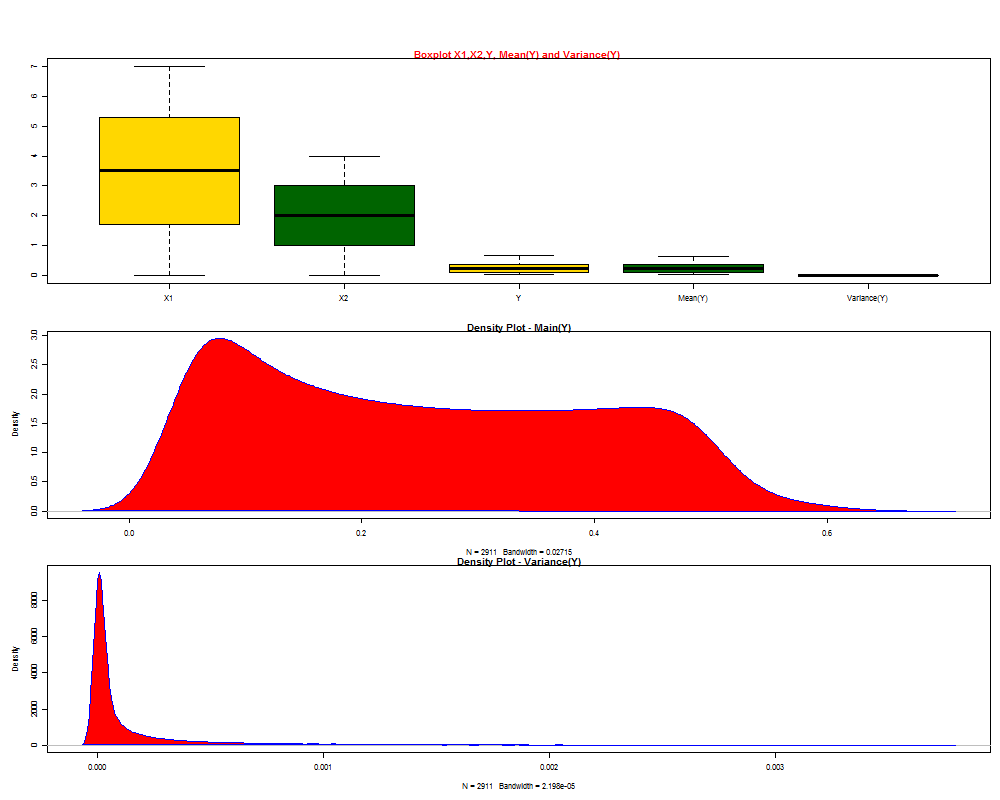
\includegraphics[scale=.50]{images/mt_train_data_anal_1.png} 
\caption{Box Plot and Density Plot of Training Data $X_1,X_2$,Mean(Y)-$\hat{\mu}$ and Variance(Y)-$\hat{\sigma}$}
\label{e_d_f_1}
\end{figure}

\FloatBarrier
\begin{figure}[!htbp]
\centering
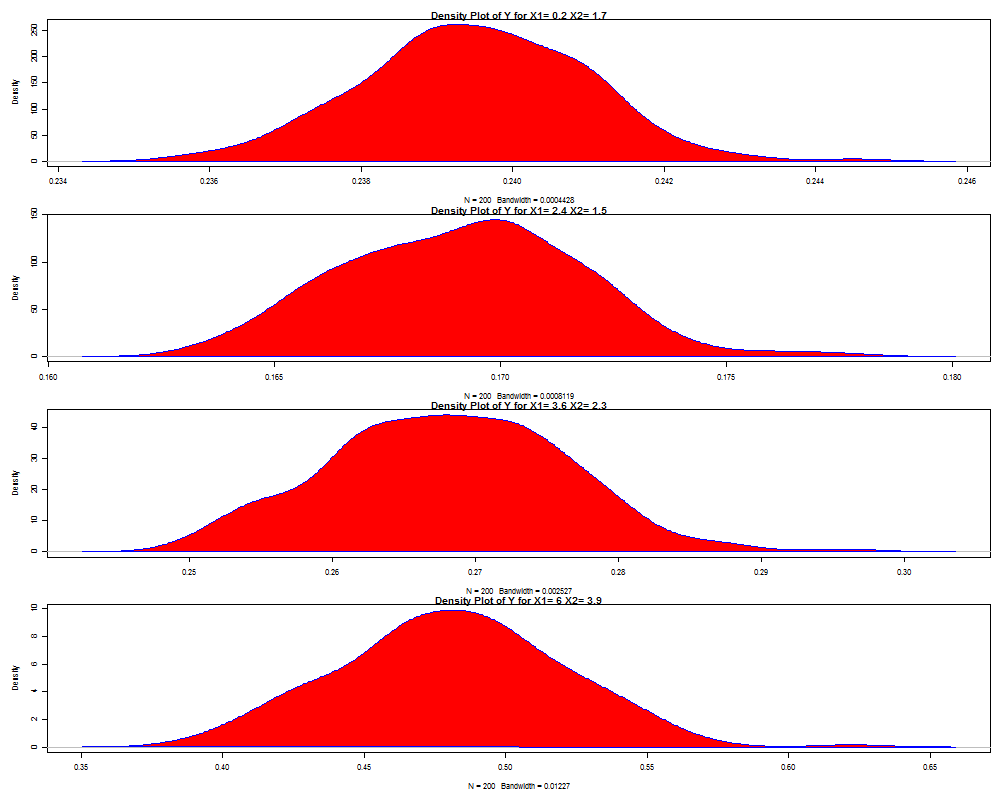
\includegraphics[scale=.43]{images/mt_train_data_anal_density_plot.png} 
\caption{Density Plot of Training Data Y for Specific $X_1,X_2$}
\label{e_d_f_2}
\end{figure}


\subsection{Correlation Analysis}

\FloatBarrier
\item
From figure $\eqref{e_d_f_3}$ Mean(Y)-$\hat{\mu}$ is strongly correlated to $X_2$ with a correlation of $\approx$ 0.99. Variance(Y)-$\hat{\sigma}$ has a moderate correlation to both $X_1,X_2$ of $\approx$ 0.5.
\begin{figure}[!htbp]
\centering
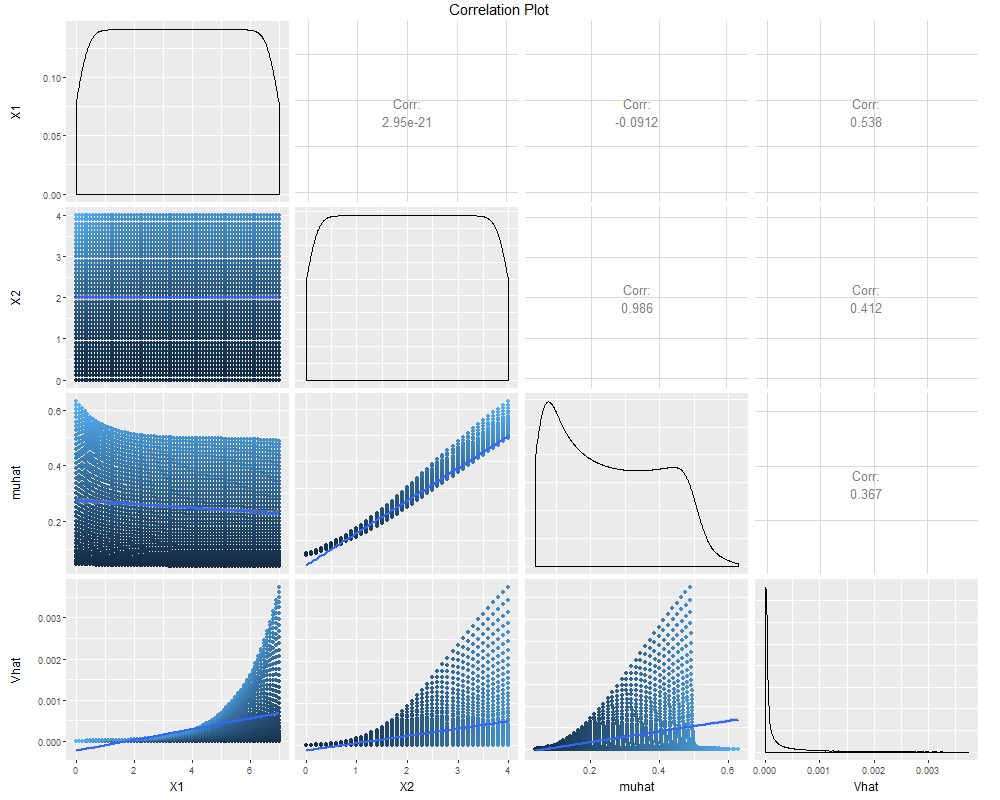
\includegraphics[scale=.43]{images/mt_ggp_corr_plot.png} 
\caption{Correlation Plot $X_1, X_2,$ Mean(Y)-$\hat{\mu}$ and Variance(Y)-$\hat{\sigma}$ with correlation values}
\label{e_d_f_3}
\end{figure}


\FloatBarrier
\subsection{Mean(Y)-$\hat{\mu}$ and Variance(Y)-$\hat{\sigma}$ Plots with $X_1,X_2$}
\item
Figure $\eqref{e_d_x_mu_var}$ plots the Mean(Y)-$\hat{\mu}$ and Variance(Y)-$\hat{\sigma}$ for $X_1$ for each value of $X_2$ and similarly for $X_2$ for each value of $X_1$.Mean(Y)-$\hat{\mu}$ appears to be independent of$X_1$ except at low values of $X_1$ between $0\dots2$. This correlation with $X_1$ is negative and very low. But correlation of  Mean(Y)-$\hat{\mu}$ with $X_2$ is very strong and increases almost linearly with $X_2$.  Variance(Y)-$\hat{\sigma}$ increases rapidly beyond  $X_1 > 5$ and $X_2 > 2$. For $X_1,X_2$ values in a range lower than this  Variance(Y)-$\hat{\sigma}$ remains low. The plot of  Mean(Y)-$\hat{\mu}$ versus $X_2$ and the plot of Variance(Y)-$\hat{\sigma}$ versus $X_1$ and $X_2$ shows patterns of a sigmoid curve.

\FloatBarrier
\begin{figure}[!htbp]
\centering
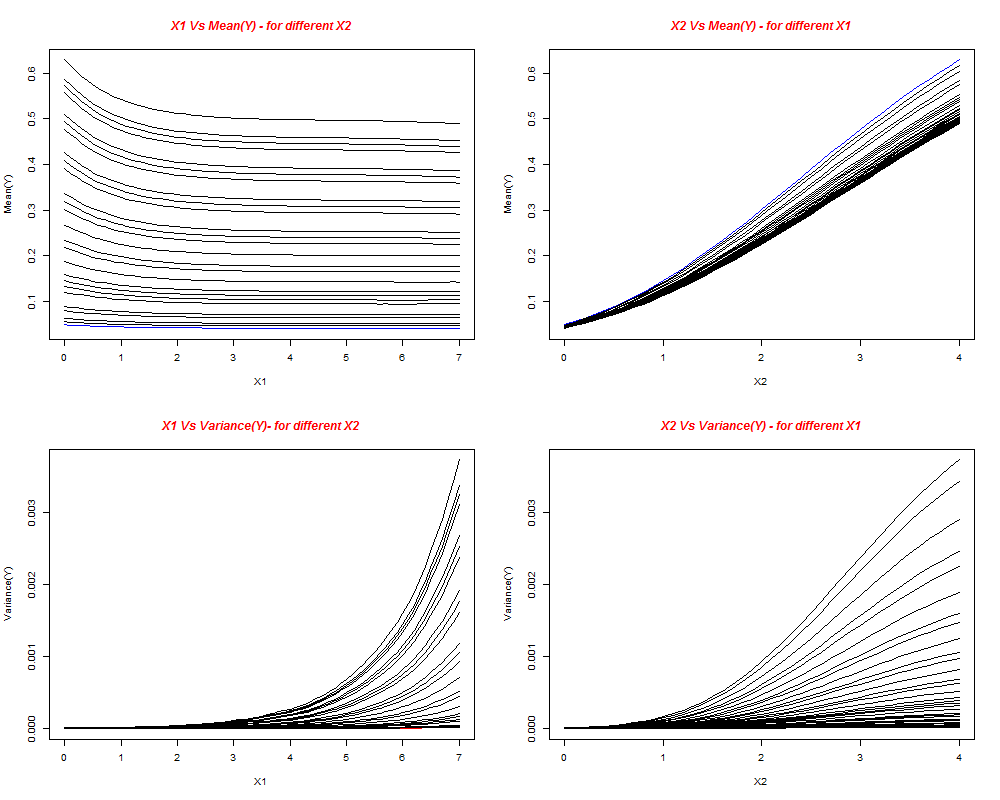
\includegraphics[scale=.50]{images/mt_scatter_detailed_plot.png} 
\caption{Detailed Correlation  $X_1, X_2,$  Mean(Y)-$\hat{\mu}$ and Variance(Y)-$\hat{\sigma}$ }
\label{e_d_x_mu_var}
\end{figure}
\FloatBarrier

\item
Figure $\eqref{e_d_mu_var_plot}$ is an interesting plot that gives us an hint on the methods that could be used for predicting Mean(Y)-$\hat{\mu}$. It plots Mean(Y)-$\hat{\mu}$ versus the variance Variance(Y)-$\hat{\sigma}$. The variance is not constant but increases and shows a wide spread as Mean(Y)-$\hat{\mu}$ increases. This indicates heteroscedasticity. 
\FloatBarrier
\begin{figure}[!htbp]
\centering
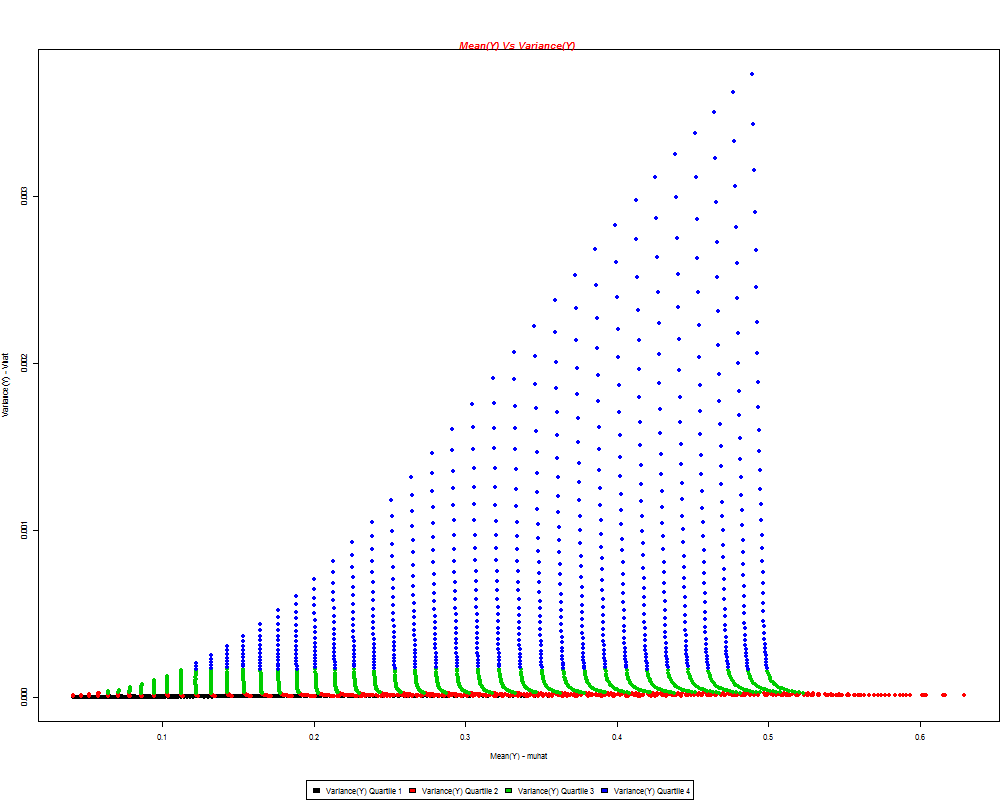
\includegraphics[scale=.50]{images/mt_matplot_mu_v_qt.png} 
\caption{ Mean(Y)-$\hat{\mu}$ Versus Variance(Y)-$\hat{\sigma}$ Plot}
\label{e_d_mu_var_plot}
\end{figure}
\FloatBarrier



\subsection{$\hat{\mu}$ and Variance(Y)-$\hat{\sigma}$ Quartile plots with $X_1,X_2$}

\FloatBarrier
\item
Figure $\eqref{e_d_f_5}$ gives a better picture of the distribution as it plots the Quartiles of Mean(Y)-$\hat{\mu}$ and Variance(Y)-$\hat{\sigma}$ simultaneously for $X_1,X_2$. The  Mean(Y)-$\hat{\mu}$ quartile bands change very little with $X_1$, but increase almost linearly with $X_2$. But the Variance(Y)-$\hat{\sigma}$ quartile bands increase for both $X_1,X2$.
\FloatBarrier
\begin{figure}[!htbp]
\centering
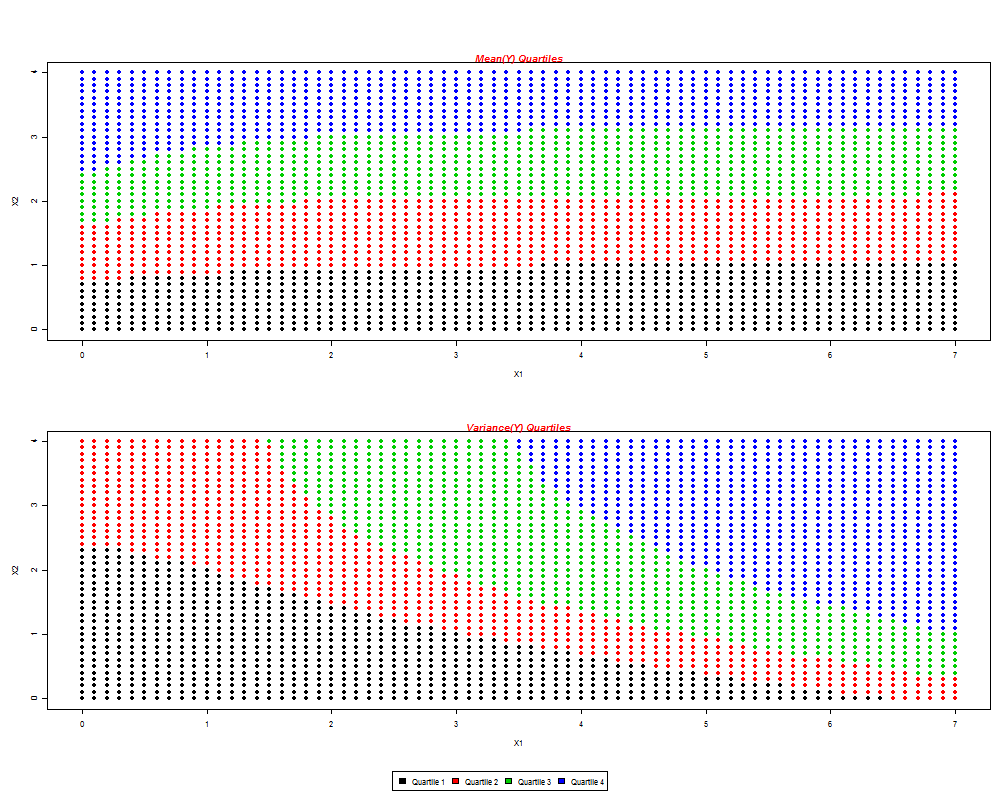
\includegraphics[scale=.50]{images/mt_matplot_x1_x2_mu_v_qt.png} 
\caption{$X_1, X_2,$ Versus  Mean(Y)-$\hat{\mu}$ and Variance(Y)-$\hat{\sigma}$ Quartile Plots}
\label{e_d_f_5}
\end{figure}

\end{itemize}








\section{Proposed Method}
\label{Proposed Method}

\subsection{Predicting Mean(Y)- $\hat{\mu}$}
From plot $\eqref{e_d_mu_var_plot}$ we see that variance is heteroscedastic and increases and widens in spread as Mean(Y)-$\hat{\mu}$ increases. Ordinary Least Squares based linear regression methods are not the best models to use in such a case as they assume homoscedasticity. We also know that Mean(Y)-$\hat{\mu}$ is in the range of $0\dots 1$. The value of Mean(Y)-$\hat{\mu}$ can be taken as P(x), the probability of success. Logistic Regression has the advantage that it does not make assumptions on the uniformity of variance nor the nature of distribution.  From the plot in $\eqref{e_d_x_mu_var}$ of Mean(Y)-$\hat{\mu}$ versus $X_2$ to which Mean(Y)-$\hat{\mu}$ is highly correlated, we can see it follows a pattern that fits the sigmoid function. So Logistic Regression model which models the sigmoid function for the response makes a nice fit for prediction of Mean(Y)-$\hat{\mu}$ based on $X_1,X_2$. Thus based on the pattern of data, Logistic Regression appears to be the best model for predicting Mean(Y)-$\hat{\mu}$. We will also explore the Linear Models so we can compare the results and choose the best model.

\subsubsection{Logistic Regression}
Here we fit a standard Logistic Regression model with Mean(Y)-$\hat{\mu}$ as response and $X_1,X_2,X_1*X_2$ as the predictor variables.

\subsubsection{Logistic Regression with Polynomial terms}
We explore the Logistic Regression model further by performing a ten fold cross validation to choose the best combination of interaction and polynomial terms of $X_1,X_2$. We will explore up-to the $6^{th}$ degree of polynomial for each predictor variable $X_1*X_2$. For each combination we will get the Cross Validation Average MSE and choose the polynomial Logistic model with the lowest Cross Validation MSE. The selected model will then be trained on the whole training data.

\subsubsection{Linear Models}
From Figure  $\eqref{e_d_f_5}$, Mean(Y)-$\hat{\mu}$ is highly positively correlated to $X_2$ and very slightly negatively correlated to low values of $X_1$. Though Logistic Regression is the first choice for predicting Mean(Y)-$\hat{\mu}$ due to reasons explained in the previous section, we will still evaluate Linear Regression models if it can add value due to this strong correlation. We will evaluate the performance of  with a regular linear regression model, a linear regression model with polynomial terms and a LASSO model with polynomial terms. The model parameters will be selected using 10 fold cross validation on the training data. Model performance will be compared using bootstrapping to select the best model for generating the test results

\paragraph{Linear Regression}
This is base model, where we try to fit a linear regression model for predicting Mean(Y)-$\hat{\mu}$ using predictor variables $X_1,X_2,X_1*X_2$

\paragraph{Linear Regression with Polynomial Terms}
Here we will use ten fold cross validation to choose the best polynomial degree for each of $X_1$ and $X_2$ for the linear regression model for predicting  Mean(Y)-$\hat{\mu}$. We propose to perform cross validation for every Polynomial combination of $X_1$ and $X_2$ to a maximum degree of 6. That gives us 36 models to choose from using ten fold cross validation for each. The model with the lowest MSE on the cross validation set is chosen. The chosen model is trained on the whole training data.

\paragraph{LASSO with Polynomial Terms}
Having linear regression with higher order polynomial terms might work well during training, but it could be picking up noise and over fitting the training data. One way to get around this while still trying to take advantage of polynomial terms to learn non linear relationships is to use a regularization model like the LASSO. LASSO has the optimization goal of minimizing the coefficients built into the learning process for building the model and so will try to shrink terms that contribute less to the model.

Here we use ten fold cross validation to again choose the best polynomial terms of $X_1$ and $X_2$ with best $\lambda$ for LASSO. The best cross validated LASSO linear regression model with the chosen polynomial terms in $X_1$ and $X_2$ is then trained on the whole training data with a further cross validation done to choose the best $\lambda$ for LASSO. The model with the chosen polynomial terms and $\lambda$ is then trained on the whole training set to get the optimum LASSO Linear Regression model.  


\subsection{Predicting Variance of Y - $\hat{\sigma}$}
From the plots $\eqref{e_d_mu_var_plot}$ we see heteroscedasticity since Variance(Y)-$\hat{\sigma}$ increases and its distribution spreads with Mean(Y)-$\hat{\mu}$ which in turn depends on $X_1,X_2$. The OLS based linear regression models assume homoscedasticity and are not a natural fit to model this pattern.From the density plots of the Variance(Y)-$\hat{\sigma}$ in  $\eqref{e_d_f_1}$ we see that Variance(Y)-$\hat{\sigma}$ has a skewed distribution with the peak very close to $0$ with a rapid fall in peak for values $>0$. We know that variance cannot be negative and in this case we know Variance(Y)-$\hat{\sigma}$ is $0 \dots 1$. So we have to fit a model where this constraint can be enforced. Any regular linear regression model fitted without enforcing this constraint might give negative values for Variance()-$\hat{\sigma}$. Negative predictions are meaningless. The plots of the Variance(Y)-$\hat{\sigma}$ versus $X_1$ and $X_2$ in 
$\eqref{e_d_x_mu_var}$ shows a pattern which is similar to the sigmoid function. Logistic Regression Model seeks to model the sigmoid function. Thus for predicting Variance(Y)-$\hat{\sigma}$ Logistic Regression Model seems to be good first first option. We will also explore the Linear Models so we can compare their performance with the Logistic Regression Models to choose the best model to be used for the test prediction of Variance(Y)-$\hat{\sigma}$. We will seek to fit the following models for prediction of Variance(Y)-$\hat{\sigma}$

\subsubsection{Logistic Regression}
We take Variance(Y)-$\hat{\sigma}$ as the P(X) value and fit a standard logistic regression model with $X_1,X_2,X_1*X_2$ as the predictors

\subsubsection{Logistic Regression with Polynomial terms}
We explore the Logistic Regression model further by performing a ten fold cross validation to choose the best combination of interaction and polynomial terms of $X_1,X_2$. We will explore up-to the $6^{th}$ degree of polynomial for each predictor variable $X_1*X_2$. For each combination we will get the Cross Validation Average MSE and from that choose the model with the lowest Cross Validation MSE.

\subsection{Linear Models}
From Figure  $\eqref{e_d_f_5}$, Variance(Y)-$\hat{\sigma}$ is correlated to both $X_1$ and $X_2$. Though Logistic Regression is the first choice for predicting Variance(Y)-$\hat{\sigma}$ due to reasons explained in the previous section, we will still evaluate the following Linear Regression models. The model parameters will be selected using 10 fold cross validation on the training data. Model performance will be compared using bootstrapping to select the best model for generating the test results


\paragraph{Linear Regression}
We take Variance()-$\hat{\sigma}$ as the response and perform a standard linear regression with $X_1,X_2,X_1*X_2$ as the predictors

\paragraph{Linear Regression with Polynomial Terms}
We will use ten fold cross validation to choose the best polynomial degree for each of $X_1$ and $X_2$ for the linear regression model for predicting Variance()-$\hat{\sigma}$. We propose to perform cross validation for every Polynomial combination of $X_1$ and $X_2$ to a maximum degree of 6. That gives us 36 models to choose from using ten fold cross validation for each. The model with the lowest MSE on the cross validation set is chosen. The chosen model is trained on the whole training data.

\paragraph{LASSO with Polynomial Terms}
Using Variance()-$\hat{\sigma}$ as the response variable we will train the LASSO model using ten fold cross validation. The first cross validation is to choose the best polynomial terms for $X_1$ and $X_2$ for the LASSO model. Once the optimum polynomial terms are chosen we perform another round of cross validation to get the best $\lambda$. The chosen model is then trained on the whole training data.







\subsection{10 Fold Cross Validation for choosing model parameters}
\begin{enumerate}
\item
The models are trained and optimum parameters for the model are chosen using the process of $10$ fold cross validation.
\item
For this purpose the training data is divided into random set of $10$ folds
\item
For cross validation all combinations of tunable parameters will be used to train the model using each set of $9$ folds as the training set and the remaining 1 fold as the test set.
\item
The average MSE across each of the 10 test folds is taken for every combination of parameters
\item
The model with the combination of parameters with the lowest average error rate is chosen as the optimum one for a given method
\item
The chosen model is trained using these optimum parameters on the whole training set
\item
The performance of the model is evaluated using bootstrapping as described next
\end{enumerate}


\subsection{Evaluating models with Bootstrapping with B=100 Iterations}

Once we have generated the different models described here, we evaluate the model using the sampling method of bootstrapping. We use all the training data for bootstrapping and perform iterations for 100 samples with replacement as follows.

\begin{itemize}
\item
A robust way to test the models is using bootstrapping. We can perform this with $B=100$ iterations
\item
Since we have sufficient data of $2911$ rows, we can pick a random $40\%$ of the data with replacement as the held back test data during each bootstrapping cycle. 
\item
Training the model on the balance $60\%$ of the data for each cycle will reduce the correlation between the models trained and thus reduce the variance on the MSE from the bootstrapping process.
\item
Using the optimum parameters we have already chosen we train each model for Mean(Y)-$\hat{\mu}$ and Variance(Y)-$\hat{\sigma}$ on the $60\%$ data designated as training data in each bootstrapping cycle. For each of the trained models we then compute the MSE as described in $\eqref{m_e_1}$ and $\eqref{m_e_2}$ on the $40\%$ data chosen as the test data. The results are tabulated for each cycle
\begin{align}
MSE_{\hat{\mu}}^{model} = \frac{1}{n} \sum_{i=1}^{i=n}  \left( \hat{\mu}_i^{test}-\hat{f}_{\hat{\mu}}^{model}\left(x_i^{test}\right) \right)^2 \label{m_e_1}\\
MSE_{\hat{\sigma}}^{model} = \frac{1}{n} \sum_{i=1}^{i=n}  \left( \hat{\sigma}_i^{test}-\hat{f}_{\hat{\sigma}}^{model}\left(x_i^{test}\right) \right)^2 \label{m_e_2}
\end{align}
\item
Once the 100 bootstrapping iterations are completed, the mean and variance of these $MSE_{\hat{\mu}}^{model}$ and $MSE_{\hat{\sigma}}^{model}$ results from each cycle for each model is computed
\item
We can now perform a statistical test like T Test or a W Test to reliably choose the best model
\item
The best model is used to predict the results on the test data set provided
\end{itemize}




\section{Results and Observations}
\label{Results and Observations}

The following are the results from cross validation and training the models.
\subsection{Predicting Mean of Y - $\hat{\mu}$}

\subsubsection{Logistic Regression}
\begin{itemize}
\item
The very low P-value for $X_2$ shows that $X_2$ is important for predicting the response Mean(Y)-$\hat{\mu}$ in this model. As expected the $X_2$ has a positive coefficient that is approximately 20 times larger in magnitude than the  negative coefficient of $X_1$. So $X_2$ has a larger contribution to the response Mean(Y)-$\hat{\mu}$.
\begin{verbatim}
> summary(lr.mu.fit)

Call:
glm(formula = muhat ~ X1 * X2, family = binomial(logit), data = data0.train)

Deviance Residuals: 
      Min         1Q     Median         3Q        Max  
-0.116587  -0.039413   0.001049   0.027583   0.151184  

Coefficients:
             Estimate Std. Error z value Pr(>|z|)    
(Intercept) -2.670132   0.228276 -11.697   <2e-16 ***
X1          -0.021026   0.057231  -0.367    0.713    
X2           0.763357   0.085642   8.913   <2e-16 ***
X1:X2       -0.007681   0.021305  -0.361    0.718    
---
Signif. codes:  0 ‘***’ 0.001 ‘**’ 0.01 ‘*’ 0.05 ‘.’ 0.1 ‘ ’ 1

(Dispersion parameter for binomial family taken to be 1)

    Null deviance: 343.2493  on 2764  degrees of freedom
Residual deviance:   6.1953  on 2761  degrees of freedom
AIC: 1690.1

Number of Fisher Scoring iterations: 5

\end{verbatim}

\FloatBarrier
\item
Figure $\eqref{o_f_l_l}$ plots the fitted values for Mean(Y)-$\hat{\mu}$ against the true values. The figure also plots the standardized residuals from the model with Mean(Y)-$\hat{\mu}$  and Variance(Y)-$\hat{\sigma}$ . The plots are colored to indicate the quartiles to which the predicted Mean(Y)-$\hat{\mu}$ values belong. Ideally we should have a $45^{\circ}$ line for the true and fitted values, in this case plot appears to have a spread as the value of Mean(Y)-$\hat{\mu}$ increases .The standardized residuals also spread higher for upper quartiles of Mean(Y)-$\hat{\mu}$ 
\FloatBarrier
\begin{figure}[!htbp]
\centering
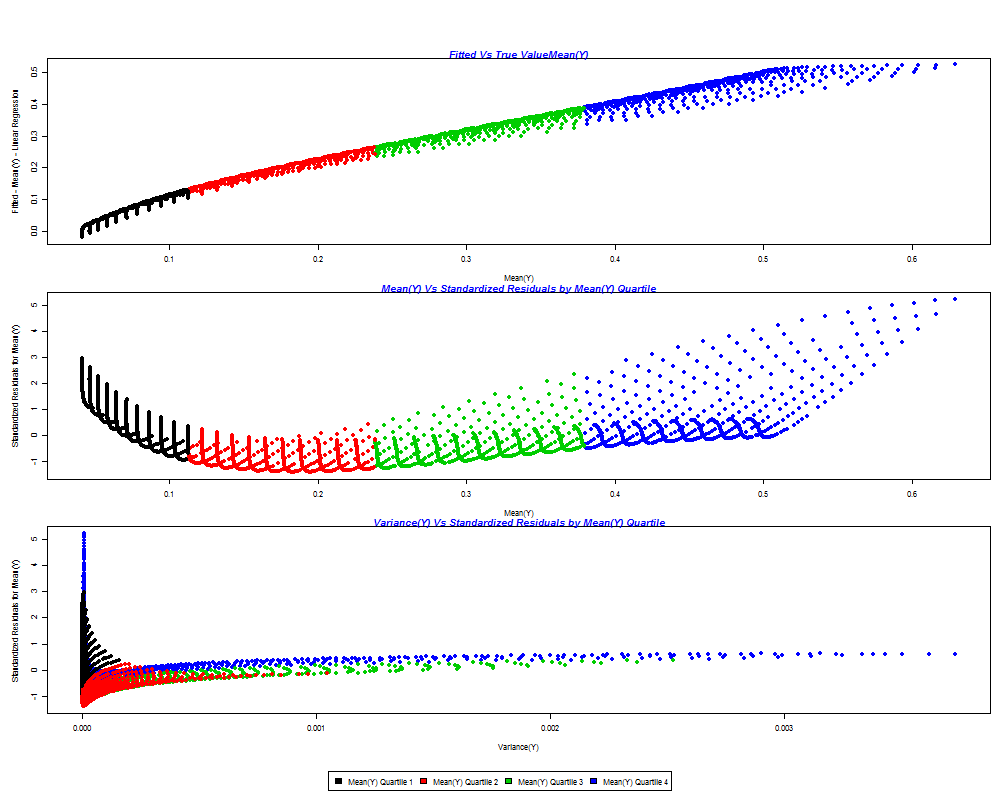
\includegraphics[scale=.50]{images/mt_rse_plot_mean_trg_slg.png} 
\caption{Logistic Regression Residuals for Mean(Y)-$\hat{\mu}$ colored by Mean(Y)-$\hat{\mu}$ Quartile}
\label{o_f_l_l}
\end{figure}


\end{itemize}


\FloatBarrier
\subsubsection{Logistic Regression with Polynomial Terms}
\begin{itemize}

\item
The 10 fold cross validation plot for MSE for various combinations of polynomial degree terms of $X_1,X2$ is shown in figure $\eqref{o_f_l_2}$. The ten fold cross validation picks degree 6 for the interaction of $X_1,X_2$ as the best model. 

\FloatBarrier
\begin{figure}[!htbp]
\centering
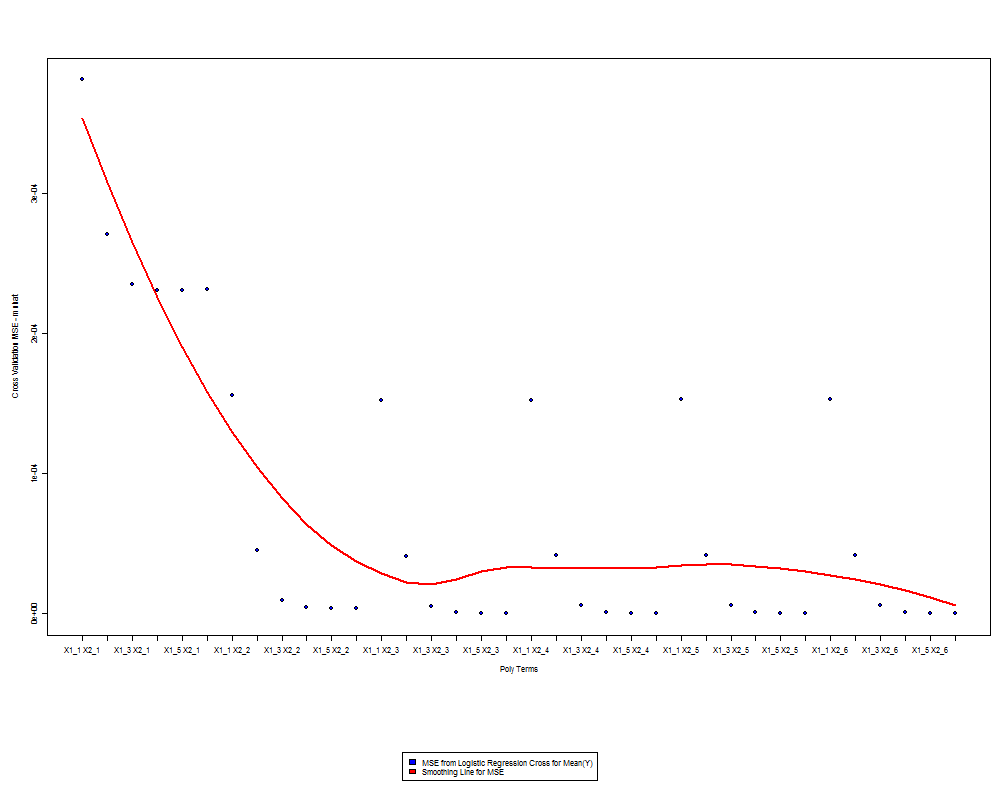
\includegraphics[scale=.43]{images/mt_cvplot_mu_lg_poly.png} 
\caption{Cross Validation MSE for predicting Mean(Y)-$\hat{\mu}$ plotted against Predictor Combinations}
\label{o_f_l_2}
\end{figure}

\item
For the best model chosen, the very low P-value for $X_2$ shows that $X_2$ is important for predicting the response Mean(Y)-$\hat{\mu}$ in this model. As expected the $X_2$ has the largest positive coefficient, so $X_2$ has a larger contribution to the response $\hat{\mu}$. The model also has a very low residual deviance of 1.1517e-04. This indicates a good fit.
\FloatBarrier
\begin{verbatim}
> summary(lrp.mu.fit)

Call:
glm(formula = muhat ~ poly(X1, poly.lrp.muhat.min.x1) * poly(X2, 
    poly.lrp.muhat.min.x2), family = binomial(logit), data = data0.train)

Deviance Residuals: 
       Min          1Q      Median          3Q         Max  
-1.010e-03  -9.421e-05   2.210e-06   9.125e-05   8.068e-04  

Coefficients:
                                                                    Estimate Std. Error z value Pr(>|z|)    
(Intercept)                                                        -1.305596   0.054222 -24.079   <2e-16 ***
poly(X1, poly.lrp.muhat.min.x1)1                                   -3.796362   2.826687  -1.343   0.1793    
poly(X1, poly.lrp.muhat.min.x1)2                                    2.571445   2.824391   0.910   0.3626    
poly(X1, poly.lrp.muhat.min.x1)3                                   -1.365234   2.831218  -0.482   0.6297    
poly(X1, poly.lrp.muhat.min.x1)4                                    0.496035   2.830411   0.175   0.8609    
poly(X1, poly.lrp.muhat.min.x1)5                                   -0.154637   2.832497  -0.055   0.9565    
poly(X1, poly.lrp.muhat.min.x1)6                                    0.043054   2.830903   0.015   0.9879    
poly(X2, poly.lrp.muhat.min.x2)1                                   48.534772   3.225216  15.049   <2e-16 ***
poly(X2, poly.lrp.muhat.min.x2)2                                   -5.942285   3.165320  -1.877   0.0605 .  
poly(X2, poly.lrp.muhat.min.x2)3                                    0.725413   3.134814   0.231   0.8170    
poly(X2, poly.lrp.muhat.min.x2)4                                   -0.048707   3.108795  -0.016   0.9875    
poly(X2, poly.lrp.muhat.min.x2)5                                    0.014232   3.015889   0.005   0.9962    
poly(X2, poly.lrp.muhat.min.x2)6                                   -0.005096   2.741535  -0.002   0.9985    
poly(X1, poly.lrp.muhat.min.x1)1:poly(X2, poly.lrp.muhat.min.x2)1 -52.359326 168.106431  -0.311   0.7554    
poly(X1, poly.lrp.muhat.min.x1)2:poly(X2, poly.lrp.muhat.min.x2)1  32.558110 167.783176   0.194   0.8461    
.
.
poly(X1, poly.lrp.muhat.min.x1)2:poly(X2, poly.lrp.muhat.min.x2)6   0.029088 142.904974   0.000   0.9998    
poly(X1, poly.lrp.muhat.min.x1)3:poly(X2, poly.lrp.muhat.min.x2)6  -0.012942 143.546195   0.000   0.9999    
poly(X1, poly.lrp.muhat.min.x1)4:poly(X2, poly.lrp.muhat.min.x2)6   0.009426 143.317540   0.000   0.9999    
poly(X1, poly.lrp.muhat.min.x1)5:poly(X2, poly.lrp.muhat.min.x2)6  -0.012221 143.219037   0.000   0.9999    
poly(X1, poly.lrp.muhat.min.x1)6:poly(X2, poly.lrp.muhat.min.x2)6  -0.003717 143.421379   0.000   1.0000    
---
Signif. codes:  0 ‘***’ 0.001 ‘**’ 0.01 ‘*’ 0.05 ‘.’ 0.1 ‘ ’ 1

(Dispersion parameter for binomial family taken to be 1)

    Null deviance: 3.4325e+02  on 2764  degrees of freedom
Residual deviance: 1.1517e-04  on 2716  degrees of freedom
AIC: 1781.5

Number of Fisher Scoring iterations: 6

\end{verbatim}

\FloatBarrier
\item
Figure $\eqref{o_f_l_3}$ plots the fitted values for Mean(Y)-$\hat{\mu}$ against the true values. The figure also plots the standardized residuals from the model with Mean(Y)-$\hat{\mu}$ and Variance(Y)-$\hat{\sigma}$. The plots are colored to indicate the quartiles to which the predicted Mean(Y)-$\hat{\mu}$ values belong. Ideally we should have a $45^{\circ}$ line for the true and fitted values, in this case the line appears to be almost ideal. The standardized residuals show a slight spread higher for upper quartiles of Mean(Y)-$\hat{\mu}$ and as Variance(Y)-$\hat{\sigma}$ increases.
\FloatBarrier
\begin{figure}[!htbp]
\centering
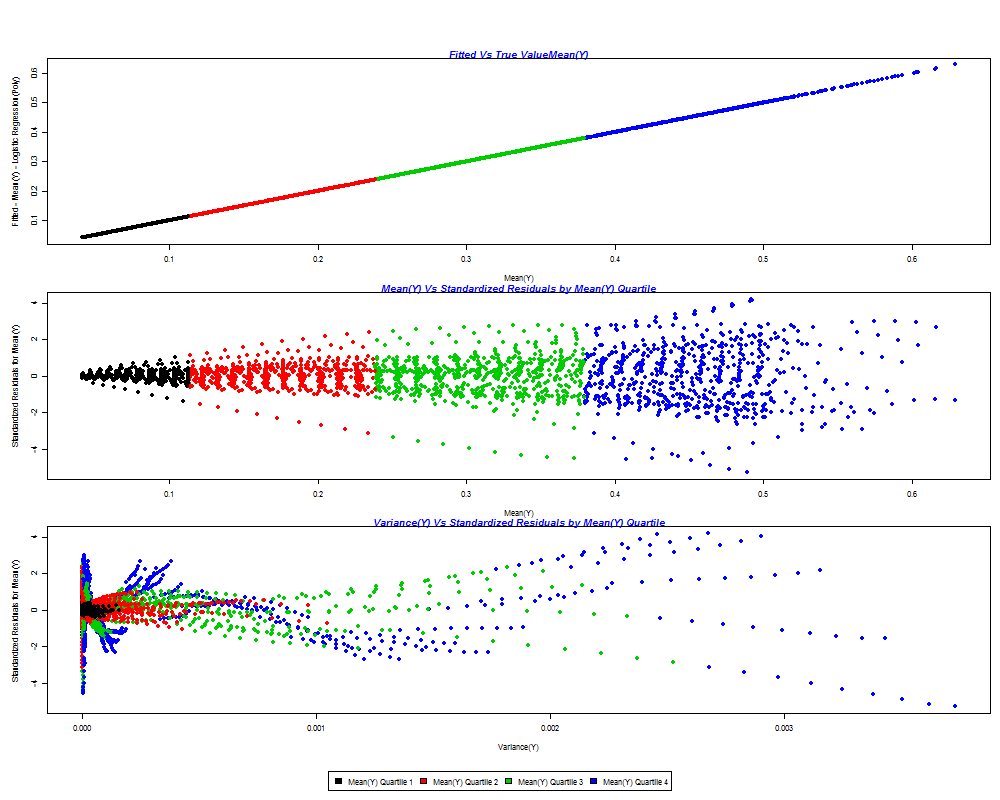
\includegraphics[scale=.50]{images/mt_rse_plot_mean_trg_lr_poly.png} 
\caption{Logistic Regression Residuals for Mean(Y)-$\hat{\mu}$ colored by Mean(Y)-$\hat{\mu}$ Quartile}
\label{o_f_l_3}
\end{figure}


\end{itemize}


\FloatBarrier
\subsubsection{Linear Methods}
\paragraph{Linear Regression}
\begin{itemize}
\item
The very low P-value for both the predictors shows that $X_1,X_2$ are important for predicting the response $\hat{\mu}$. As expected the $X_2$ has a positive coefficient that is approximately 20 times larger in magnitude than the  negative coefficient of $X_1$. So $X_2$ has a larger contribution to the response $\hat{\mu}$.
\begin{verbatim}
> summary(lm.mu.fit)

Call:
lm(formula = muhat ~ X1 + X2, data = data0.train)

Residuals:
      Min        1Q    Median        3Q       Max 
-0.028385 -0.013942 -0.003463  0.008320  0.106545 

Coefficients:
              Estimate Std. Error t value Pr(>|t|)    
(Intercept)  0.0269571  0.0010017   26.91   <2e-16 ***
X1          -0.0065778  0.0001885  -34.90   <2e-16 ***
X2           0.1238886  0.0003272  378.69   <2e-16 ***
---
Signif. codes:  0 ‘***’ 0.001 ‘**’ 0.01 ‘*’ 0.05 ‘.’ 0.1 ‘ ’ 1

Residual standard error: 0.02037 on 2762 degrees of freedom
Multiple R-squared:  0.9812,    Adjusted R-squared:  0.9812 
F-statistic: 7.223e+04 on 2 and 2762 DF,  p-value: < 2.2e-16
\end{verbatim}

\FloatBarrier
\item
Figure $\eqref{o_f_l}$ plots the fitted values for Mean(Y)-$\hat{\mu}$ against the true values. The figure also plots the standardized residuals from the model with Mean(Y)-$\hat{\mu}$ and Variance(Y)-$\hat{\sigma}$. The plots are colored to indicate the quartiles to which the predicted Mean(Y)-$\hat{\mu}$ values belong. Ideally we should have a $45^{\circ}$ line for the true and fitted values,the fit for this model seem moderate. The standardized residuals show a slight spread higher for upper quartiles of Mean(Y)-$\hat{\mu}$ but remain constant as Variance(Y)-$\hat{\sigma}$ increases.
\FloatBarrier
\begin{figure}[!htbp]
\centering
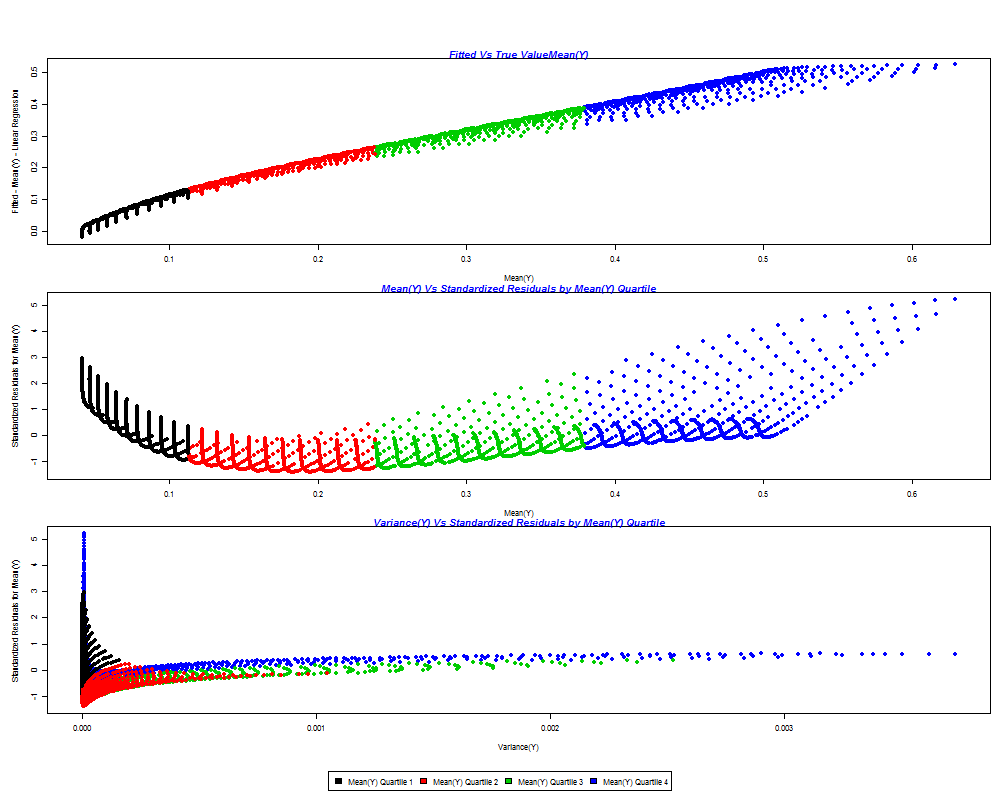
\includegraphics[scale=.50]{images/mt_rse_plot_mean_trg_slg.png} 
\caption{Linear Regression Residuals for Mean(Y)-$\hat{\mu}$ colored by Mean(Y)-$\hat{\mu}$  Quartile}
\label{o_f_l}
\end{figure}
\end{itemize}



\FloatBarrier
\paragraph{Linear Regression with Polynomial Terms}
\begin{itemize}
\item
The 10 fold cross validation to choose the optimum polynomial degree terms of $X_1,X_1$ chooses degree 5 for $X_1$ and degree 5 for $X_2$. The predictor terms with degree $1\dots 4$ of $X_1$ and degree $1 \dots 3$ of $X_2$ have a very low P-value, so these predictors $X_1,X_1^2,X_1^3,X_1^4,X_2,X_2^2,X_2^3$ are important for predicting the response Mean(Y)-$\hat{\mu}$. As expected the $X_2$ has a positive coefficient that is approximately 10 times larger in magnitude than the next largest coefficient. So $X_2$ has a larger contribution to the response Mean(Y)-$\hat{\mu}$. An $R^2=.99$ shows the model explains most of the variance seen in the response Mean(Y)-$\hat{\mu}$. The $R^2=.99$ for this model is slightly higher than the $R^2=.98$ for the previous discussed standard Linear Regression Model.
\begin{verbatim}
> summary(lmp.mu.fit)

Call:
lm(formula = muhat ~ poly(X1, poly.muhat.min.x1) + poly(X2, poly.muhat.min.x2), 
    data = data0.train)

Residuals:
      Min        1Q    Median        3Q       Max 
-0.055339 -0.004731  0.000045  0.004683  0.053252 

Coefficients:
                              Estimate Std. Error  t value Pr(>|t|)    
(Intercept)                   0.250342   0.000191 1310.527  < 2e-16 ***
poly(X1, poly.muhat.min.x1)1 -0.712481   0.010045  -70.927  < 2e-16 ***
poly(X1, poly.muhat.min.x1)2  0.481318   0.010045   47.916  < 2e-16 ***
poly(X1, poly.muhat.min.x1)3 -0.268686   0.010045  -26.748  < 2e-16 ***
poly(X1, poly.muhat.min.x1)4  0.103488   0.010046   10.301  < 2e-16 ***
poly(X1, poly.muhat.min.x1)5 -0.032485   0.010045   -3.234  0.00124 ** 
poly(X2, poly.muhat.min.x2)1  7.713699   0.010045  767.882  < 2e-16 ***
poly(X2, poly.muhat.min.x2)2  0.680636   0.010045   67.759  < 2e-16 ***
poly(X2, poly.muhat.min.x2)3 -0.295859   0.010046  -29.452  < 2e-16 ***
poly(X2, poly.muhat.min.x2)4 -0.010412   0.010045   -1.037  0.30003    
poly(X2, poly.muhat.min.x2)5  0.022359   0.010045    2.226  0.02611 *  
---
Signif. codes:  0 ‘***’ 0.001 ‘**’ 0.01 ‘*’ 0.05 ‘.’ 0.1 ‘ ’ 1

Residual standard error: 0.01004 on 2754 degrees of freedom
Multiple R-squared:  0.9955,    Adjusted R-squared:  0.9954 
F-statistic: 6.029e+04 on 10 and 2754 DF,  p-value: < 2.2e-16

\end{verbatim}

\FloatBarrier
\item
Figure $\eqref{o_f_2}$ plots the fitted values for Mean(Y)-$\hat{\mu}$ against the true values. The figure also plots the standardized residuals from the model with Mean(Y)-$\hat{\mu}$ and Variance(Y)-$\hat{\sigma}$. The plots are colored to indicate the quartiles to which the predicted Mean(Y)-$\hat{\mu}$ values belong. Ideally we should have a $45^{\circ}$ line for the true and fitted values,the fit for this model seems good. The standardized residuals show a slight spread higher for upper quartiles of Mean(Y)-$\hat{\mu}$ but remain constant as Variance(Y)-$\hat{\sigma}$ increases.
\FloatBarrier
\begin{figure}[!htbp]
\centering
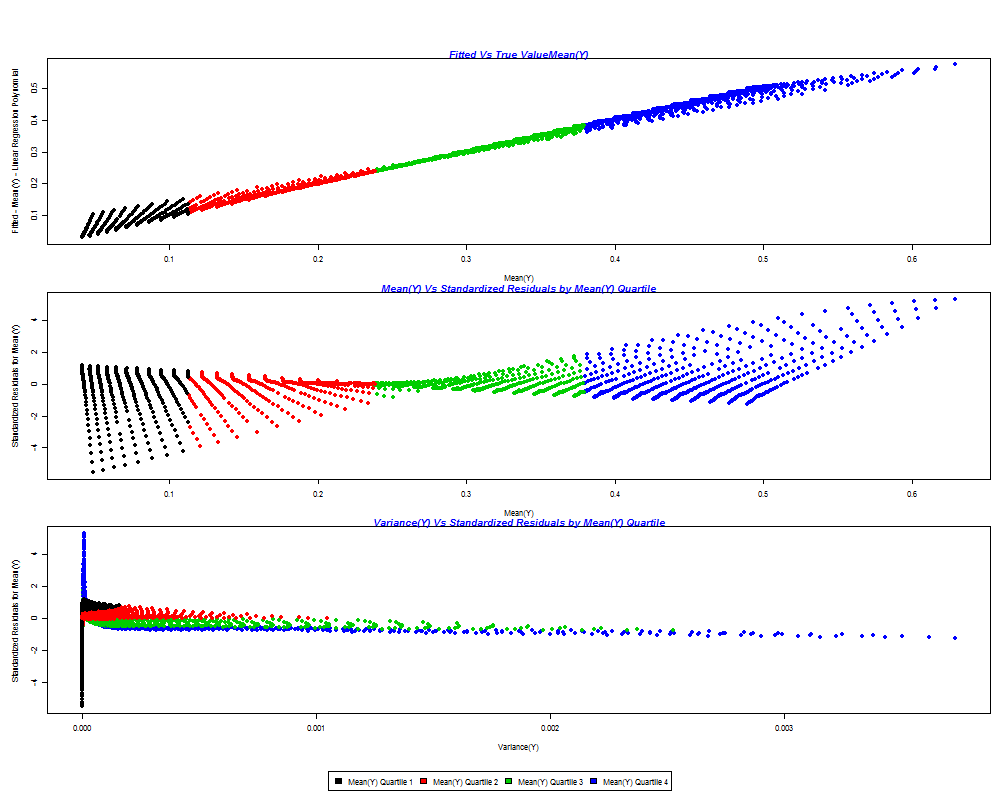
\includegraphics[scale=.50]{images/mt_rse_plot_mean_trg_lg_poly.png} 
\caption{Linear Regression (Polynomial) Residuals for Mean(Y)-$\hat{\mu}$ colored by Mean(Y)-$\hat{\mu}$ Quartile}
\label{o_f_2}
\end{figure}


\end{itemize}





\FloatBarrier
\paragraph{LASSO with Polynomial Terms}
\begin{itemize}

\item
The 10 fold cross validation to choose the optimum polynomial degree terms of $X_1,X_1$ for LASSO, along with a further ten fold validation to choose the best $\lambda$ for these polynomial terms yields an value of $\lambda=1.429932e-05$. The cross validation plot for LASSO plotting MSE for various values of $\lambda$ is in figure $\eqref{o_f_4}$ and shows the best $\lambda$ value after which we see a sharp upward elbow in MSE.
\FloatBarrier
\begin{figure}[!htbp]
\centering
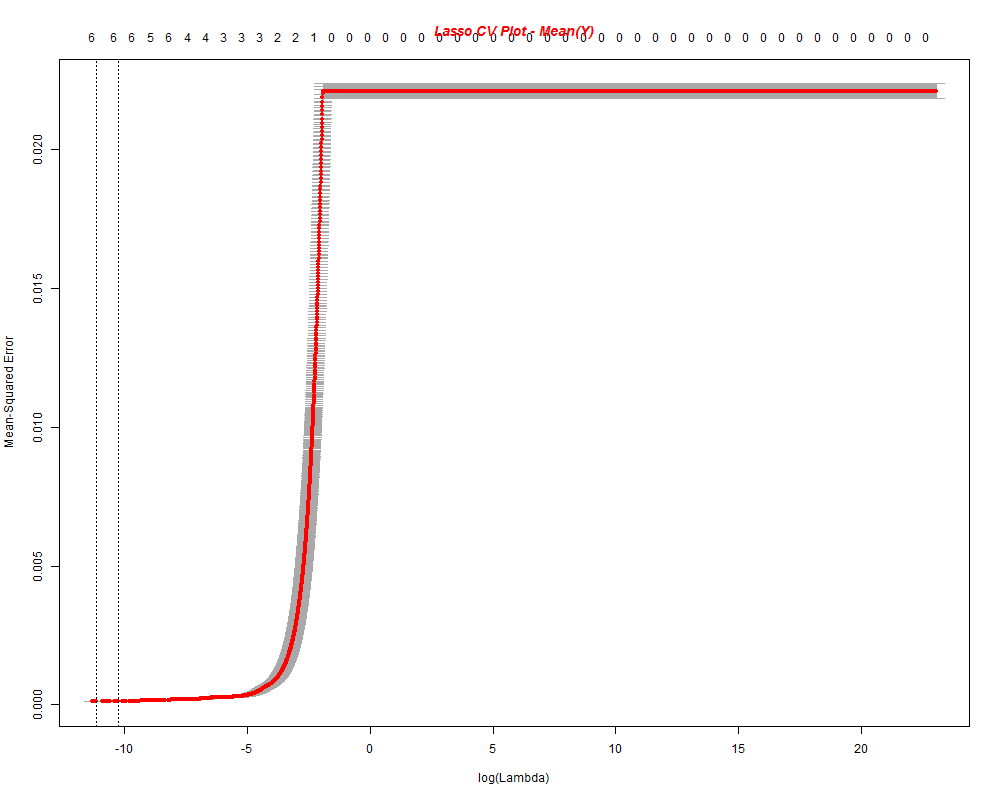
\includegraphics[scale=.50]{images/lasso_cv_plot_mean.png} 
\caption{LASSO (Polynomial) Cross Validation Plot for Mean(Y)-$\hat{\mu}$ for choosing $\lambda$}
\label{o_f_4}
\end{figure}

\FloatBarrier
\item
The chosen $\lambda$ shrinks the coefficients for several polynomial terms of $X_1,X_2$, choosing only $X_1,X_1^2,X_1^3,X_2,X_2^2,X_2^4$. However in contrast to the previously discussed Linear Regression with polynomial terms, the coefficients have been reduced in magnitude for $X_1,X_2$ by a tenth. The coefficient of $X_2$ is just slightly higher than the magnitude of the coefficient for $X_1$ and $X_2^2$ has a coefficient of almost equal in magnitude to $X_1$. The $R^2=.9953$ computed for this model is slightly higher than the $R^2=.98$ for the previous discussed standard Linear Regression Model.
\begin{verbatim}
> lasso.muhat.bestlam
[1] 1.429932e-05
>
>
> coef(lasso.mu.fit, s = "lambda.min")
8 x 1 sparse Matrix of class "dgCMatrix"
                        1
(Intercept)  0.0917578311
X1          -0.0384341029
X2           0.0529331096
X2.1         0.0078598984
X3          -0.0005229176
X2.2         0.0244319522
X3.1         .           
X4.1        -0.0005124043

\end{verbatim}

\FloatBarrier
\item
Figure $\eqref{o_f_3}$ plots the fitted values for Mean(Y)-$\hat{\mu}$ against the true values. The figure also plots the standardized residuals from the model with Mean(Y)-$\hat{\mu}$ and Variance(Y)-$\hat{\sigma}$. The plots are colored to indicate the quartiles to which the predicted Mean(Y)-$\hat{\mu}$ values belong. Ideally we should have a $45^{\circ}$ line for the true and fitted values,the fit for this model seems very good. The standardized residuals show a slight spread higher for upper quartiles of Mean(Y)-$\hat{\mu}$ but remain constant as Variance(Y)-$\hat{\sigma}$ increases.
\FloatBarrier
\begin{figure}[!htbp]
\centering
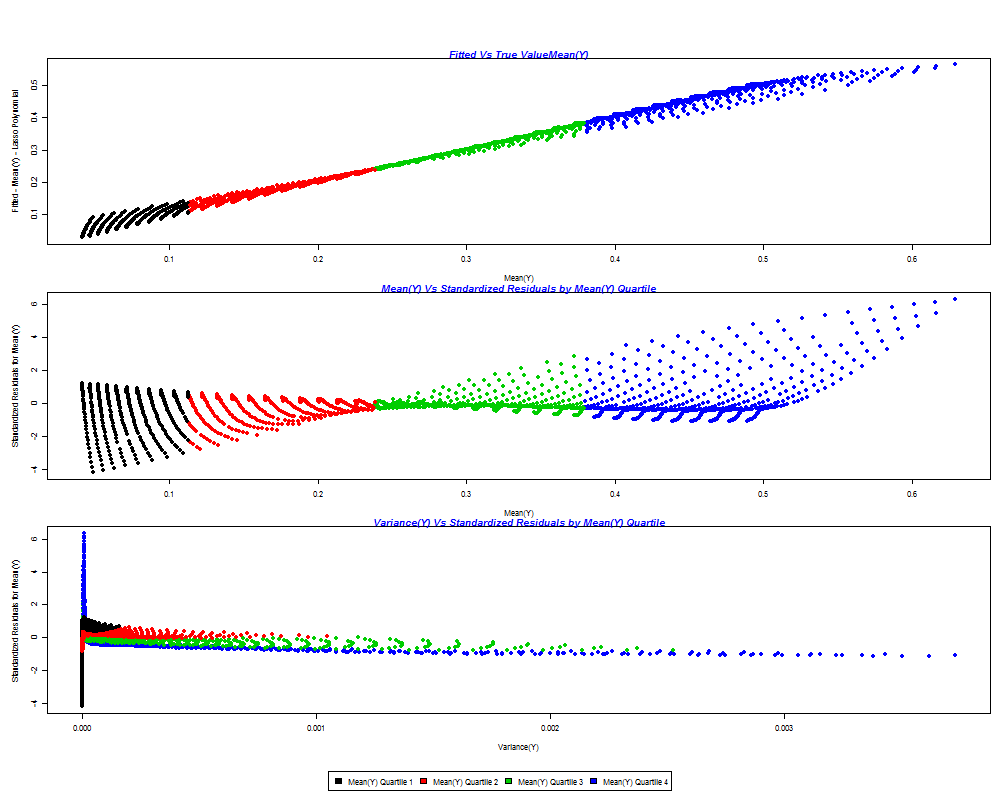
\includegraphics[scale=.50]{images/mt_rse_plot_mean_trg_lasso_poly.png} 
\caption{LASSO (Polynomial) Residuals for  Mean(Y)-$\hat{\mu}$  colored by Mean(Y)-$\hat{\mu}$ Quartile}
\label{o_f_3}
\end{figure}



\end{itemize}







\FloatBarrier
\subsection{Predicting Variance of Y - $\hat{\sigma}$}

\subsubsection{Logistic Regression}
\begin{itemize}
\item
The P-Values of the coefficients are not very significant indicating that the predictors are not strong contributors to the response. The Residual deviance is low.
\begin{verbatim}
> summary(lr.v.fit)

Call:
glm(formula = Vhat ~ X1 * X2, family = binomial(logit), data = data0.train)

Deviance Residuals: 
       Min          1Q      Median          3Q         Max  
-0.0199292  -0.0021285  -0.0003975   0.0009398   0.0101573  

Coefficients:
              Estimate Std. Error z value Pr(>|z|)
(Intercept) -1.524e+01  2.574e+01  -0.592    0.554
X1           8.855e-01  4.262e+00   0.208    0.835
X2           9.451e-01  8.055e+00   0.117    0.907
X1:X2       -4.239e-04  1.333e+00   0.000    1.000

(Dispersion parameter for binomial family taken to be 1)

    Null deviance: 1.696732  on 2764  degrees of freedom
Residual deviance: 0.043195  on 2761  degrees of freedom
AIC: 9.2597

Number of Fisher Scoring iterations: 14



\end{verbatim}

\FloatBarrier
\item
Figure $\eqref{o_f_vl_l}$ plots the fitted values for Variance(Y)-$\hat{\sigma}$ against the true values. The figure also plots the standardized residuals from the model with Mean(Y)-$\hat{\mu}$  and Variance(Y)-$\hat{\sigma}$ . The plots are colored to indicate the quartiles to which the predicted Variance(Y)-$\hat{\sigma}$ values belong. Ideally we should have a $45^{\circ}$ line for the true and fitted values, in this case plot appears to have a spread as the value of Mean(Y)-$\hat{\mu}$ increases. The model appears to underestimate Variance(Y)-$\hat{\sigma}$. The standardized residuals also spread lower for upper quartiles of Variance(Y)-$\hat{\sigma}$ 
\FloatBarrier
\begin{figure}[!htbp]
\centering
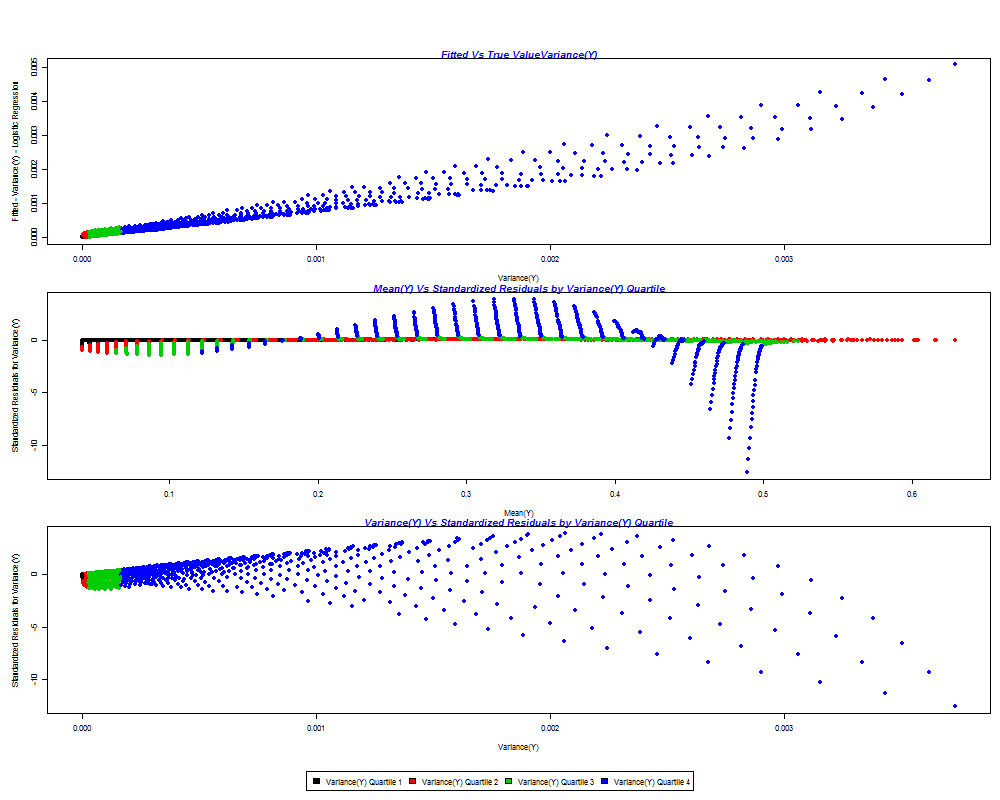
\includegraphics[scale=.50]{images/mt_rse_plot_v_trg_lr.png} 
\caption{Logistic Regression Residuals for Variance(Y)-$\hat{\sigma}$ colored by Variance(Y)-$\hat{\sigma}$ Quartile}
\label{o_f_vl_l}
\end{figure}


\end{itemize}


\FloatBarrier
\subsubsection{Logistic Regression with Polynomial Terms}
\begin{itemize}
\FloatBarrier
\item
The 10 fold cross validation plot for MSE for various combinations of polynomial degree terms of $X_1,X2$ is shown in figure $\eqref{o_f_vl_2}$. The ten fold cross validation picks degree 4 for the interaction of $X_1,X_2$ as the best model. 

\FloatBarrier
\begin{figure}[!htbp]
\centering
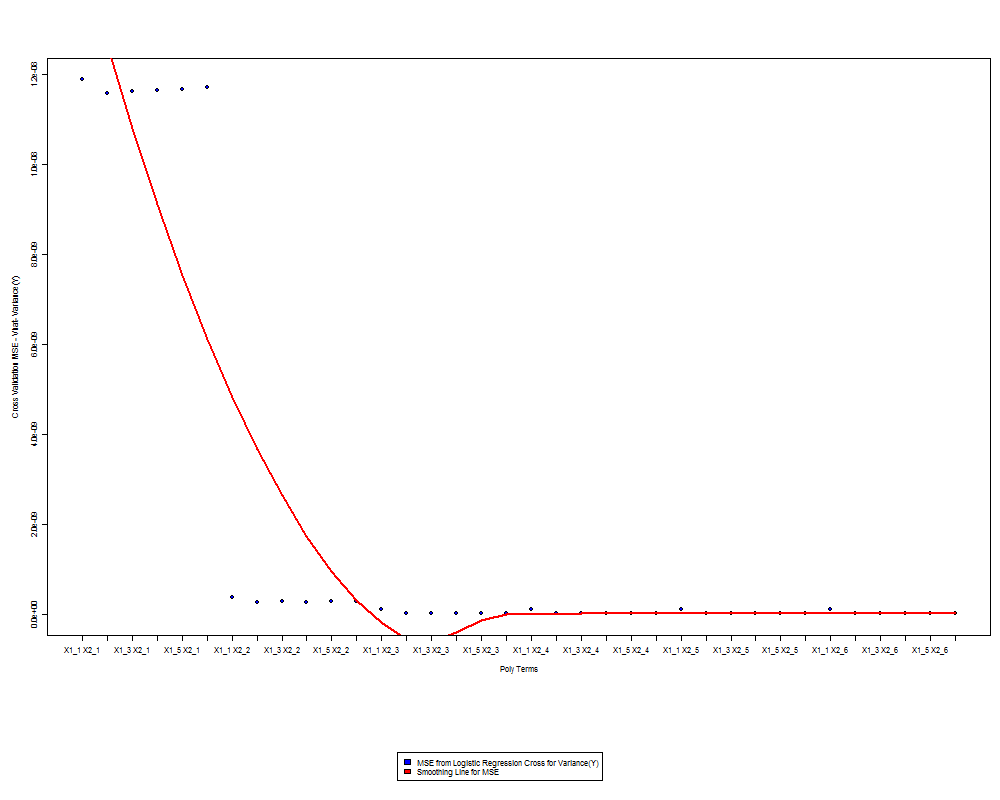
\includegraphics[scale=.50]{images/mt_cvplot_v_lg_poly.png} 
\caption{Cross Validation MSE for predicting Variance(Y)-$\hat{\sigma}$ plotted against Predictor Combinations}
\label{o_f_vl_2}
\end{figure}

\item
The P-values of the coefficients are not very significant, indicating that the any single predictor itself is not a very strong contributor to the Variance(Y)-$\hat{\sigma}$ response in this model. The model also has a very low residual deviance of 5.1198e-05. This indicates a good fit.
\FloatBarrier
\begin{verbatim}
> summary(lrp.v.fit)

Call:
glm(formula = Vhat ~ poly(X1, poly.lrp.vhat.min.x1) * poly(X2, 
    poly.lrp.vhat.min.x2), family = binomial(logit), data = data0.train)

Deviance Residuals: 
       Min          1Q      Median          3Q         Max  
-6.831e-04  -5.645e-05  -1.440e-06   5.897e-05   4.655e-04  

Coefficients:
                                                                  Estimate Std. Error z value Pr(>|z|)
(Intercept)                                                     -1.069e+01  1.658e+01  -0.645    0.519
poly(X1, poly.lrp.vhat.min.x1)1                                  9.506e+01  1.075e+03   0.088    0.930
poly(X1, poly.lrp.vhat.min.x1)2                                  2.842e+00  9.944e+02   0.003    0.998
poly(X1, poly.lrp.vhat.min.x1)3                                 -3.002e+00  8.527e+02  -0.004    0.997
poly(X1, poly.lrp.vhat.min.x1)4                                  9.794e-01  4.727e+02   0.002    0.998
poly(X2, poly.lrp.vhat.min.x2)1                                  9.098e+01  1.218e+03   0.075    0.940
poly(X2, poly.lrp.vhat.min.x2)2                                 -2.918e+01  1.129e+03  -0.026    0.979
poly(X2, poly.lrp.vhat.min.x2)3                                  4.658e+00  8.387e+02   0.006    0.996
poly(X2, poly.lrp.vhat.min.x2)4                                 -3.724e-01  4.616e+02  -0.001    0.999
poly(X1, poly.lrp.vhat.min.x1)1:poly(X2, poly.lrp.vhat.min.x2)1  9.928e+01  7.904e+04   0.001    0.999
poly(X1, poly.lrp.vhat.min.x1)2:poly(X2, poly.lrp.vhat.min.x2)1 -1.051e+02  7.310e+04  -0.001    0.999
poly(X1, poly.lrp.vhat.min.x1)3:poly(X2, poly.lrp.vhat.min.x2)1  1.416e+01  6.264e+04   0.000    1.000
poly(X1, poly.lrp.vhat.min.x1)4:poly(X2, poly.lrp.vhat.min.x2)1  2.414e+00  3.469e+04   0.000    1.000
poly(X1, poly.lrp.vhat.min.x1)1:poly(X2, poly.lrp.vhat.min.x2)2  3.491e+01  7.331e+04   0.000    1.000
poly(X1, poly.lrp.vhat.min.x1)2:poly(X2, poly.lrp.vhat.min.x2)2 -7.987e+00  6.774e+04   0.000    1.000
poly(X1, poly.lrp.vhat.min.x1)3:poly(X2, poly.lrp.vhat.min.x2)2  1.638e+01  5.799e+04   0.000    1.000
poly(X1, poly.lrp.vhat.min.x1)4:poly(X2, poly.lrp.vhat.min.x2)2 -7.784e+00  3.205e+04   0.000    1.000
poly(X1, poly.lrp.vhat.min.x1)1:poly(X2, poly.lrp.vhat.min.x2)3 -1.324e+01  5.468e+04   0.000    1.000
poly(X1, poly.lrp.vhat.min.x1)2:poly(X2, poly.lrp.vhat.min.x2)3  6.697e+00  5.054e+04   0.000    1.000
poly(X1, poly.lrp.vhat.min.x1)3:poly(X2, poly.lrp.vhat.min.x2)3 -6.783e-01  4.304e+04   0.000    1.000
poly(X1, poly.lrp.vhat.min.x1)4:poly(X2, poly.lrp.vhat.min.x2)3  6.267e-01  2.368e+04   0.000    1.000
poly(X1, poly.lrp.vhat.min.x1)1:poly(X2, poly.lrp.vhat.min.x2)4  1.583e+00  3.052e+04   0.000    1.000
poly(X1, poly.lrp.vhat.min.x1)2:poly(X2, poly.lrp.vhat.min.x2)4 -7.899e-01  2.817e+04   0.000    1.000
poly(X1, poly.lrp.vhat.min.x1)3:poly(X2, poly.lrp.vhat.min.x2)4 -7.512e-01  2.355e+04   0.000    1.000
poly(X1, poly.lrp.vhat.min.x1)4:poly(X2, poly.lrp.vhat.min.x2)4  1.268e-02  1.275e+04   0.000    1.000

(Dispersion parameter for binomial family taken to be 1)

    Null deviance: 1.6967e+00  on 2764  degrees of freedom
Residual deviance: 5.1198e-05  on 2740  degrees of freedom
AIC: 51.26

Number of Fisher Scoring iterations: 18


\end{verbatim}

\FloatBarrier
\item
Figure $\eqref{o_f_vl_3}$ plots the fitted values for Variance(Y)-$\hat{\sigma}$ against the true values. The figure also plots the standardized residuals from the model with Mean(Y)-$\hat{\mu}$ and Variance(Y)-$\hat{\sigma}$. The plots are colored to indicate the quartiles to which the predicted Variance(Y)-$\hat{\sigma}$ values belong. Ideally we should have a $45^{\circ}$ line for the true and fitted values, in this case the line appears to be almost ideal, which is very good. The standardized residuals show a slight spread higher for upper quartiles of Mean(Y)-$\hat{\mu}$ and  Variance(Y)-$\hat{\sigma}$
\FloatBarrier
\begin{figure}[!htbp]
\centering
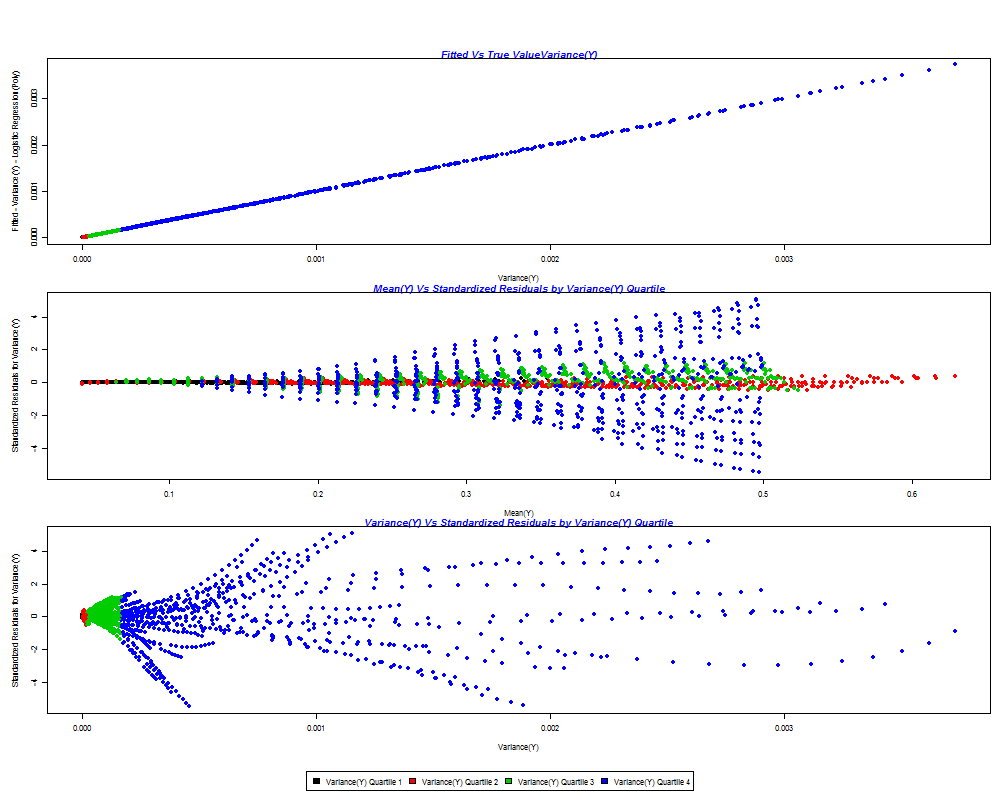
\includegraphics[scale=.50]{images/mt_rse_plot_v_trg_lr_poly.png} 
\caption{Logistic Regression Residuals for Variance(Y)-$\hat{\sigma}$ colored by Variance(Y)-$\hat{\sigma}$ Quartile}
\label{o_f_vl_3}
\end{figure}


\end{itemize}



\FloatBarrier
\subsubsection{Linear Methods}

\paragraph{Linear Regression}
\begin{itemize}
\FloatBarrier
\item
The very low P-value for both the predictors shows that $X_1,X_2$ are important for predicting the response $\hat{\sigma}$. As expected the $X_1,X_2$ have positive coefficients that are comparable in magnitude. So both predictors have a approximately similar contribution to the response $\hat{\sigma}$. However the $R^2=0.46$, is very low and indicates that the model is does a poor job of explaining away the variance seen in Variance(Y)-$\hat{\sigma}$
\begin{verbatim}
> summary(lm.v.fit)

Call:
lm(formula = Vhat ~ X1 + X2, data = data0.train)

Residuals:
       Min         1Q     Median         3Q        Max 
-4.139e-04 -2.441e-04 -9.666e-05  1.318e-04  2.690e-03 

Coefficients:
              Estimate Std. Error t value Pr(>|t|)    
(Intercept) -5.808e-04  1.819e-05  -31.93   <2e-16 ***
X1           1.310e-04  3.423e-06   38.28   <2e-16 ***
X2           1.758e-04  5.942e-06   29.58   <2e-16 ***
---
Signif. codes:  0 ‘***’ 0.001 ‘**’ 0.01 ‘*’ 0.05 ‘.’ 0.1 ‘ ’ 1

Residual standard error: 0.00037 on 2762 degrees of freedom
Multiple R-squared:  0.4603,    Adjusted R-squared:  0.4599 
F-statistic:  1178 on 2 and 2762 DF,  p-value: < 2.2e-16


\end{verbatim}

\FloatBarrier
\item
Figure $\eqref{o_f_11}$ plots the fitted values for Variance(Y)-$\hat{\sigma}$ against the true values and shows a very poor fit.  The plots for the standardized residuals from the model with Mean(Y)-$\hat{\mu}$ and Variance(Y)-$\hat{\sigma}$ show residuals increase with Variance(Y)-$\hat{\sigma}$ and spread wider with Mean(Y)-$\hat{\mu}$ for this model
\FloatBarrier
\begin{figure}[!htbp]
\centering
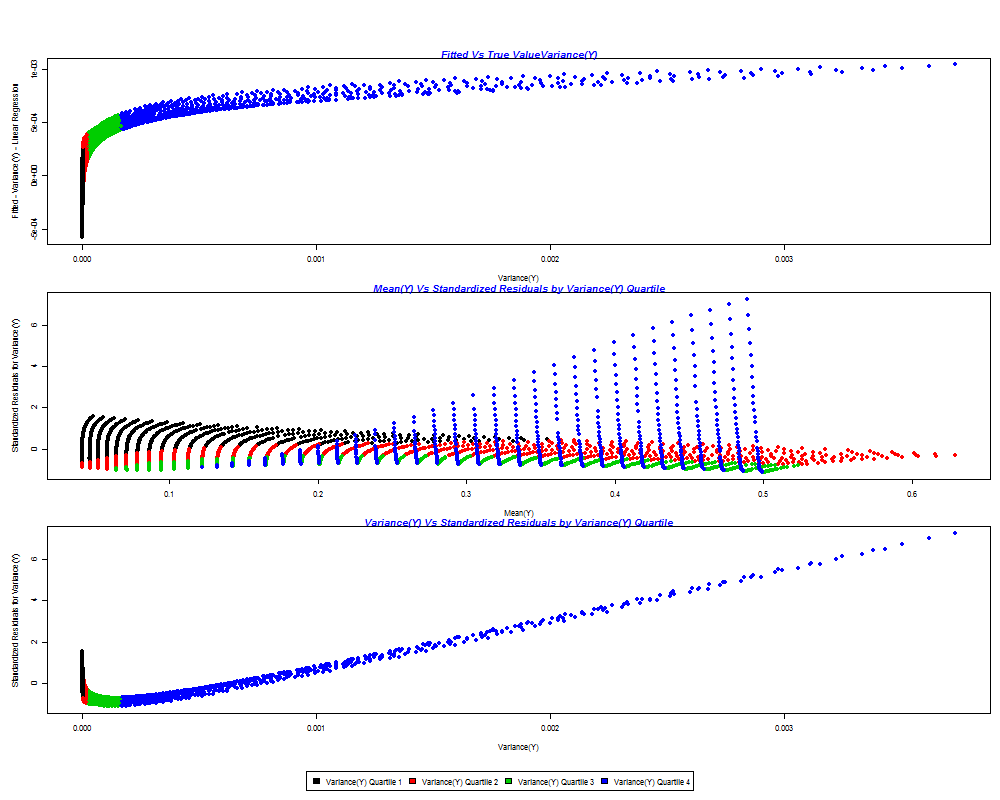
\includegraphics[scale=.50]{images/mt_rse_plot_var_v_trg_slg.png} 
\caption{Linear Regression Residuals for Variance(Y)-$\hat{\sigma}$  colored by Variance(Y)-$\hat{\sigma}$  Quartile}
\label{o_f_11}
\end{figure}

\end{itemize}


\FloatBarrier
\paragraph{Linear Regression with Polynomial Terms}
\begin{itemize}
\FloatBarrier
\item
The 10 fold cross validation to choose the optimum polynomial degree terms for $X_1,X_1$ chooses degree 4 for $X_1$ and degree 4 for $X_2$. The predictor terms with degree $1\dots 3$ of $X_1$ and degree $1 \dots 2$ of $X_2$ have a very low P-value, so these predictors $X_1,X_1^2,X_1^3,X_2,X_2^2$ are important for predicting the response Variance(Y)-$\hat{\sigma}$ .As expected the terms in $X_1,X_2$ have coefficients that are comparable in magnitude. So both predictors have a approximately similar contribution to the response Variance(Y)-$\hat{\sigma}$ . An $R^2=.82$ shows the model explains only around $60\%$ of the variance seen in the response Variance(Y)-$\hat{\sigma}$ . The $R^2=.62$ for this model is slightly higher than the $R^2=.46$ for the previous discussed standard Linear Regression Model but still not very good.
\begin{verbatim}
> summary(lmp.v.fit)

Call:
lm(formula = Vhat ~ poly(X1, poly.Vhat.min.x1) + poly(X2, poly.Vhat.min.x2), 
    data = data0.train)

Residuals:
       Min         1Q     Median         3Q        Max 
-1.066e-03 -1.616e-04  1.999e-05  1.544e-04  2.013e-03 

Coefficients:
                              Estimate Std. Error t value Pr(>|t|)    
(Intercept)                  2.276e-04  5.934e-06  38.358  < 2e-16 ***
poly(X1, poly.Vhat.min.x1)1  1.416e-02  3.121e-04  45.375  < 2e-16 ***
poly(X1, poly.Vhat.min.x1)2  9.092e-03  3.121e-04  29.134  < 2e-16 ***
poly(X1, poly.Vhat.min.x1)3  4.001e-03  3.121e-04  12.821  < 2e-16 ***
poly(X1, poly.Vhat.min.x1)4  1.357e-03  3.121e-04   4.349 1.42e-05 ***
poly(X2, poly.Vhat.min.x2)1  1.091e-02  3.121e-04  34.970  < 2e-16 ***
poly(X2, poly.Vhat.min.x2)2  2.899e-03  3.121e-04   9.290  < 2e-16 ***
poly(X2, poly.Vhat.min.x2)3 -6.763e-04  3.121e-04  -2.167   0.0303 *  
poly(X2, poly.Vhat.min.x2)4 -5.100e-04  3.121e-04  -1.634   0.1023    
---
Signif. codes:  0 ‘***’ 0.001 ‘**’ 0.01 ‘*’ 0.05 ‘.’ 0.1 ‘ ’ 1

Residual standard error: 0.0003121 on 2756 degrees of freedom
Multiple R-squared:  0.617,     Adjusted R-squared:  0.6159 
F-statistic: 555.1 on 8 and 2756 DF,  p-value: < 2.2e-16


\end{verbatim}

\FloatBarrier
\item
Figure $\eqref{o_f_21}$ plots the fitted values for Variance(Y)-$\hat{\sigma}$ against the true values and shows a very poor fit.  The plots for the standardized residuals from the model with Mean(Y)-$\hat{\mu}$ and Variance(Y)-$\hat{\sigma}$ show residuals increase with Variance(Y)-$\hat{\sigma}$ and spread wider with Mean(Y)-$\hat{\mu}$ for this model
\FloatBarrier
\begin{figure}[!htbp]
\centering
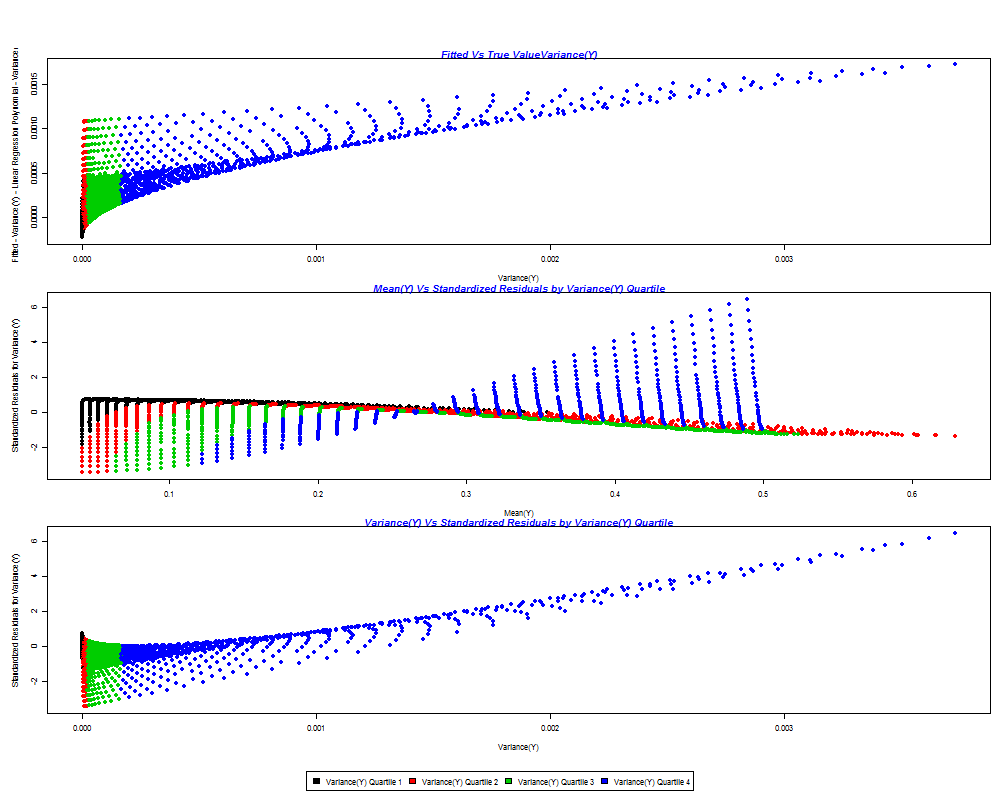
\includegraphics[scale=.50]{images/mt_rse_plot_var_v_trg_lg_poly.png} 
\caption{Linear Regression (Polynomial) Residuals for Variance(Y)-$\hat{\sigma}$  colored by Variance(Y)-$\hat{\sigma}$  Quartile}
\label{o_f_21}
\end{figure}

\end{itemize}


\FloatBarrier
\paragraph{LASSO with Polynomial Terms}

\begin{itemize}
\FloatBarrier
\item
The 10 fold cross validation to choose the optimum polynomial degree terms of $X_1,X_1$ for LASSO, along with a further ten fold validation to choose the best $\lambda$ for these polynomial terms yields an value of $\lambda=1.429932e-05$. The cross validation plot for LASSO plotting MSE for various values of $\lambda$ is in figure $\eqref{o_f_41}$ and shows the best $\lambda$ value after which we see a sharp upward elbow in MSE.
\FloatBarrier
\begin{figure}[!htbp]
\centering
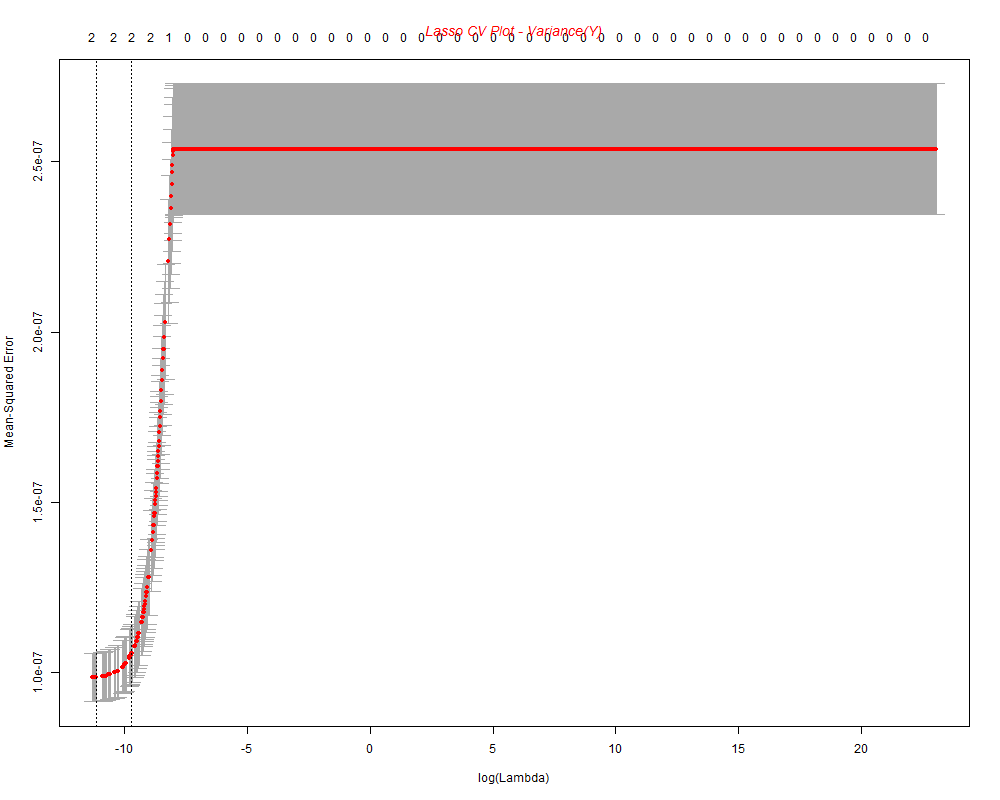
\includegraphics[scale=.50]{images/lasso_cv_plot_v.png} 
\caption{LASSO (Polynomial) Cross Validation Plot for Variance(Y)-$\hat{\sigma}$ for choosing $\lambda$}
\label{o_f_41}
\end{figure}

\FloatBarrier
\item
The chosen $\lambda$ shrinks the coefficients for several polynomial terms of $X_1,X_2$, choosing only $X_1^5,X_2^2$. However in contrast to the previously discussed Linear Regression with polynomial terms, The coefficients have been vastly reduced in magnitude. The coefficient of $X_2^2$ is just  higher than the magnitude of the coefficient for $X_1^5$.The $R^2=.61$ for this model is only slightly higher than the $R^2=.46$ for the previous discussed standard Linear Regression Model.

\begin{verbatim}
> lasso.Vhat.bestlam
[1] 1.429932e-05



> coef(lasso.v.fit, s = "lambda.min")
8 x 1 sparse Matrix of class "dgCMatrix"
                        1
(Intercept) -2.022018e-04
X1           .           
X2           .           
X2.1         .           
X3           .           
X4           .           
X5           7.202326e-08
X2.2         4.118209e-05

> print(lasso.Vhat.R.squared)
[1] 0.61413

\end{verbatim}

\FloatBarrier
\item
Figure $\eqref{o_f_31}$ the plot of the fitted values for Variance(Y)-$\hat{\sigma}$ against the true values again shows a very poor fit.  The plots for the standardized residuals from the model with Mean(Y)-$\hat{\mu}$ and Variance(Y)-$\hat{\sigma}$ show residuals increase with Variance(Y)-$\hat{\sigma}$ and spread wider with Mean(Y)-$\hat{\mu}$ for this model
\FloatBarrier
\begin{figure}[!htbp]
\centering
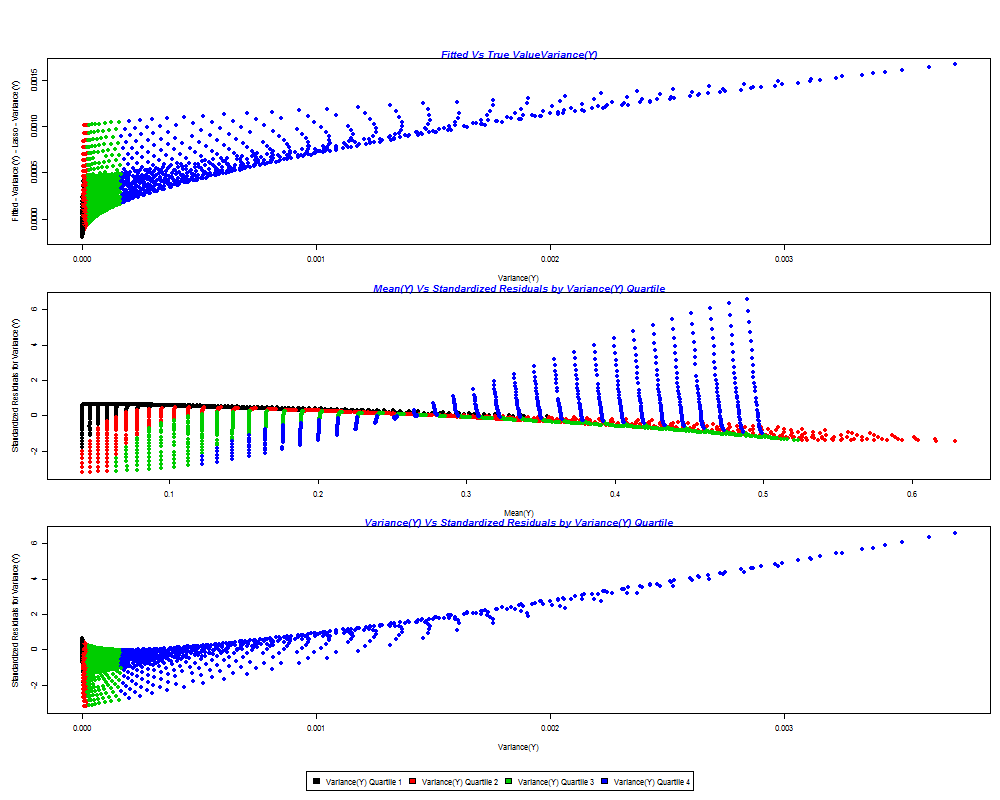
\includegraphics[scale=.50]{images/mt_rse_plot_var_v_trg_lasso_poly.png} 
\caption{LASSO (Polynomial) Residuals for  Variance(Y)-$\hat{\sigma}$ colored by Variance(Y)-$\hat{\sigma}$ Quartile}
\label{o_f_31}
\end{figure}


\end{itemize}





















\FloatBarrier
\section{Test Results}
\subsection{Cross Validation Results}
\begin{itemize}
\FloatBarrier
\item
The following table $\eqref{cv_tab_1}$ tabulates the optimum parameters and predictors chosen for each of the models for predicting Mean(Y)-$\hat{\mu}$ and  Variance(Y)-$\hat{\sigma}$. These optimum parameters are picked after 10 fold cross validation from a pool of various candidate models. The models are chosen based on the lowest average MSE.
\begin{table}[h]
\centering
\resizebox{\textwidth}{!}{
	\begin{tabular}{|c|c|c|c|c|c|c|c|c|c|c|}
		\hline
		&\multicolumn{5}{|c|}{Mean(Y)}&\multicolumn{5}{|c|}{Variance(Y)}\\
		\hline
		& Logistic Regression(LR) & LR (Polynomial) & Linear Regression (LM) & LM (Polynomial) & LASSO(Poly) & LR & LR(Poly )& LM & LM(Poly) & LASSO(Poly) \\
		\hline
		 Predictors Used &  \begin{tabular}{@{}c@{}}$X_1$\\$X_2$\end{tabular} &  \begin{tabular}{@{}c@{}}$X_1 \dots X_1^6$\\$X_2 \dots X_2^6$\end{tabular} & \begin{tabular}{@{}c@{}}$X_1$\\$X_2$\end{tabular} & \begin{tabular}{@{}c@{}}Poly($X_1$,5)\\Poly($X_2$,5)\end{tabular} & \begin{tabular}{@{}c@{}}$X_1,X_1^2,X_1^3$\\$X_2,X_2^2,X_2^4$ \end{tabular}&   \begin{tabular}{@{}c@{}}$X_1$\\$X_2$\end{tabular}& \begin{tabular}{@{}c@{}}$X_1 \dots X_1^4$\\$X_2 \dots X_2^4$\end{tabular} &\begin{tabular}{@{}c@{}}$X_1$\\$X_2$\end{tabular} &  \begin{tabular}{@{}c@{}}Poly($X_1$,4)\\Poly($X_2$,4)\end{tabular} & \begin{tabular}{@{}c@{}}$X_1^5$\\$X_2^2$ \end{tabular} \\
		\hline
		 Parameters Used & & &  &  & $\lambda$ =1.43e-05 &  & & & & $\lambda$ = 1.43e-05 \\
		 \hline
	\end{tabular}
	}
	\caption[]{Parameters and Predictors chosen for models by 10 fold cross validation}
	\label{cv_tab_1}
\end{table}
\end{itemize}

\FloatBarrier
\subsection{Bootstrapping 100 Iterations Test Results}
\begin{itemize}

\FloatBarrier
\item
Tables $\eqref{bs_tab_1}$ and $\eqref{bs_tab_11}$ tabulate the bootstrapping results from 100 iterations for both Mean(Y)-$\hat{\mu}$ and  Variance(Y)-$\hat{\sigma}$ predictions.  Bootstrapping is performed using the optimum models chosen by cross validation. The table shows Average MSE and the variance in MSE for each model across 100 bootstrapping iterations. The results are for models predicting both the Mean(Y)-$\hat{\mu}$ and  Variance(Y)-$\hat{\sigma}$.
\begin{table}[h]
	\centering
	\resizebox{\textwidth}{!}{
		\begin{tabular}{|c|c|c|c|c|c|}
			\hline
			& Logistic Regression & Logistic Regression with Polynomial Terms & Linear Regression & Linear Regression with Polynomial terms & LASSO(Pol)\\
			\hline
			Average MSE(Mean(Y))       & 0.0003824652 &  1.017951e-08 &  0.0004166204  &  0.00010101&  0.0001077252\\
			\hline
			Variance MSE(Mean(Y))      &  3.720936e-10  & 4.794325e-19  & 6.280023e-10  & 5.819501e-11 & 8.059884e-11\\
			\hline
		\end{tabular}
	}
	\caption[]{Bootstrapping results for the models evaluated for predicting Mean(Y)-$\hat{\mu}$}
	\label{bs_tab_1}
\end{table}

\FloatBarrier
\begin{table}[h]
	\centering
	\resizebox{\textwidth}{!}{
		\begin{tabular}{|c|c|c|c|c|c|}
			\hline
			& Logistic Regression & Logistic Regression with Poly Terms & Linear Regression & Linear Regression with Poly terms & LASSO(Poly)\\
			\hline
			Average MSE(Variance(Y))       &  1.12547e-08  & 7.419421e-12  & 1.330242e-07 & 9.554755e-08 & 9.58125e-08\\
			\hline
			Variance MSE(Variance(Y))      &  4.471789e-18   &      4.082094e-25    &  1.376597e-16  &  5.702572e-17 & 6.542574e-17 \\
			\hline
		\end{tabular}
	}
	\caption[]{Bootstrapping results for the models evaluated for predicting  Variance(Y)-$\hat{\sigma}$}
	\label{bs_tab_11}
\end{table}

\item
Figure $\eqref{bs_f_1}$ box plots the MSE from each of the 100 bootstrap iterations for both the Mean(Y)-$\hat{\mu}$ and Variance(Y)-$\hat{\sigma}$ predictor models. The box plot shows the variance from each model.
\FloatBarrier
\begin{figure}[!htbp]
	\centering
	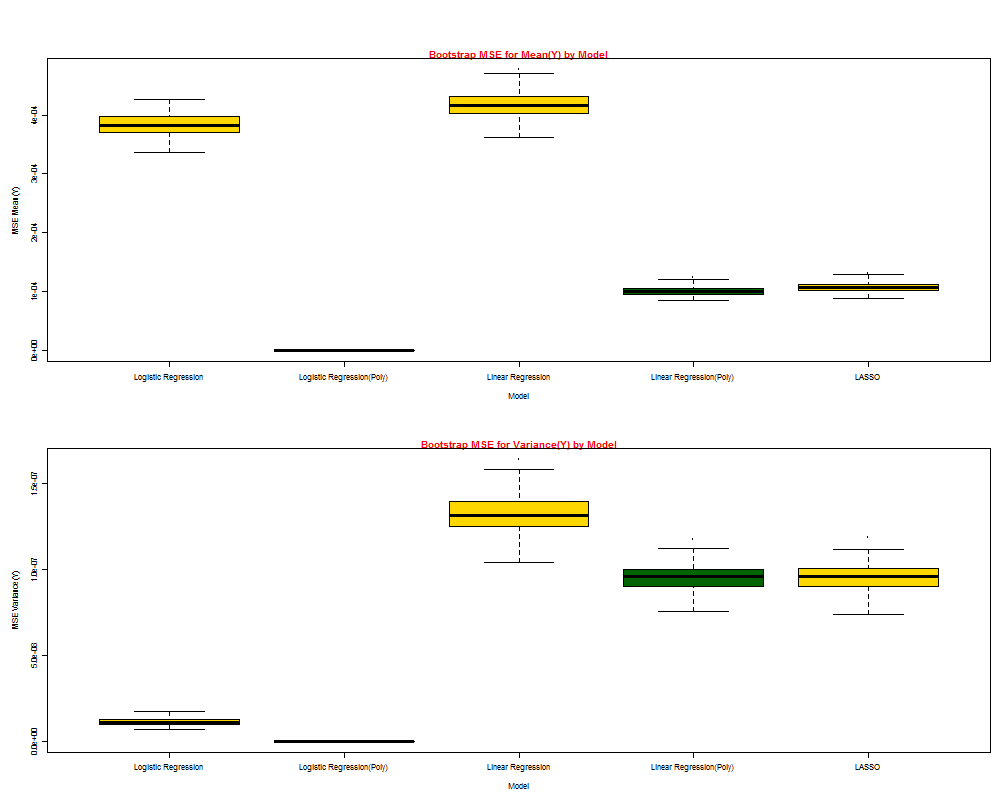
\includegraphics[scale=.50]{images/mt_boxplot_bootstrap_muhat_results.png} 
	\caption{Box-plot of Bootstrapping MSE results of both  Mean(Y)-$\hat{\mu}$ and  Variance(Y)-$\hat{\sigma}$ predictor models}
	\label{bs_f_1}
\end{figure}


\FloatBarrier
\item
Figure $\eqref{bs_f_2}$ summarizes the bootstrap results for each model predicting  Mean(Y)-$\hat{\mu}$ by plotting the average MSE and Variance in MSE. 
\begin{figure}[!htbp]
\centering
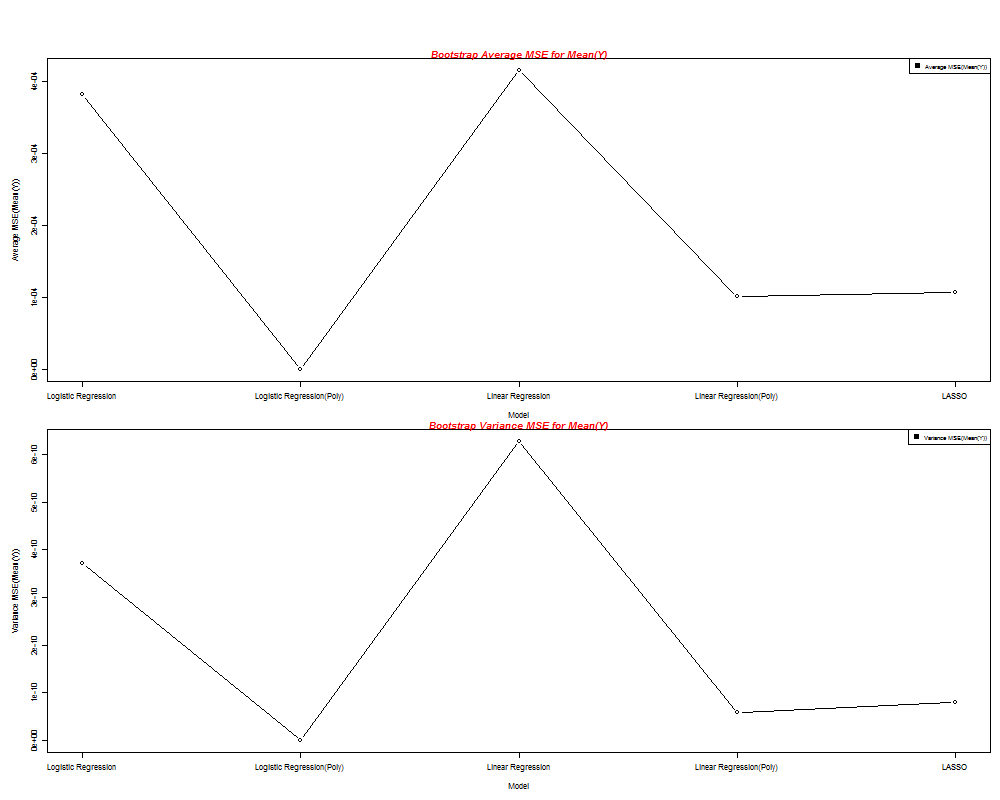
\includegraphics[scale=.50]{images/mt_bootstrap_muhat_mse_var_plot.png} 
\caption{Bootstrapping 100 Iterations - Average MSE , Variance MSE for the  Mean(Y)-$\hat{\mu}$ prediction models}
\label{bs_f_2}
\end{figure}


\FloatBarrier
\item
Figure $\eqref{bs_f_3}$ summarizes the bootstrap results for each model predicting Variance(Y)-$\hat{\sigma}$ by plotting the average MSE and Variance in MSE. 
\begin{figure}[!htbp]
	\centering
	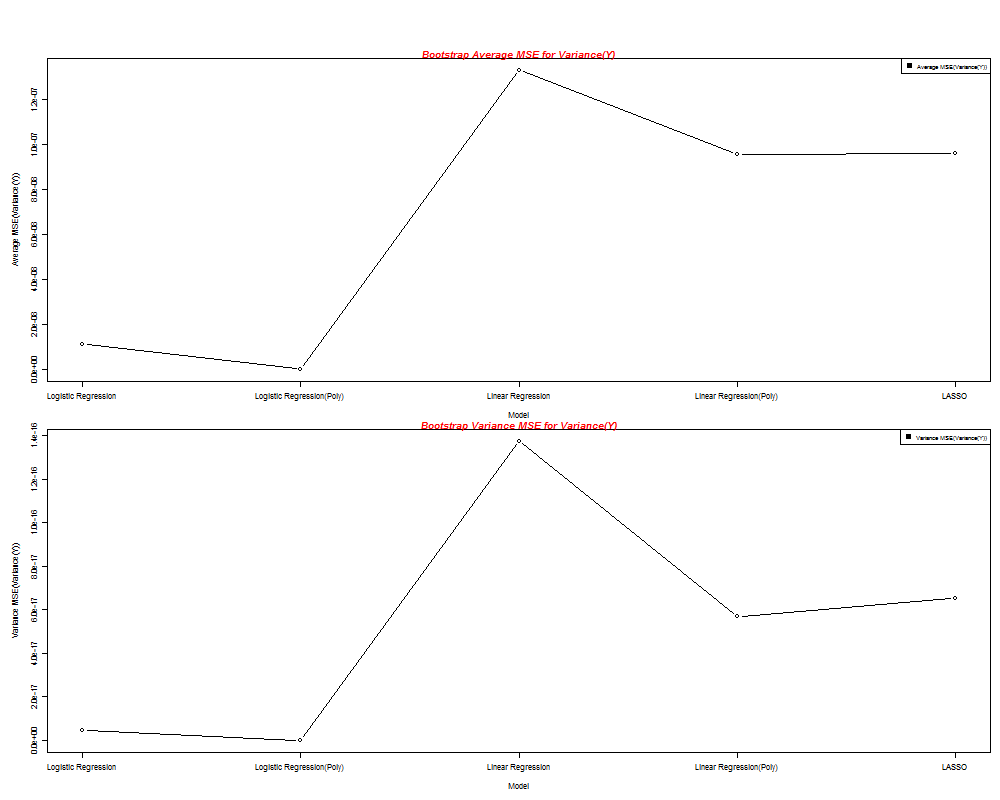
\includegraphics[scale=.50]{images/mt_bootstrap_vhat_mse_var_plot.png} 
	\caption{Bootstrapping 100 Iterations - Average MSE , Variance MSE for the Variance(Y)-$\hat{\sigma}$ prediction models}
	\label{bs_f_3}
\end{figure}


\end{itemize}


\FloatBarrier
\subsection{T-test and Wilcox Test for  Mean(Y)-$\hat{\mu}$ prediction models}
\begin{itemize}
	\item
	From the bootstrapping MSE results for the  Mean(Y)-$\hat{\mu}$ predictor methods in table $\eqref{bs_tab_1}$ and the plot in $\eqref{bs_f_2}$ The polynomial Logistic Regression Model has the lowest average MSE and variance in MSE.
	\item
	We run a T Test and a Wilcox test on these bootstrapping MSE with the null hypothesis $H_0$ that these models are statistically similar at the $\alpha = 5\%$ significance. The MSE from Polynomial Logistic Regression is compared to the MSE from other two models in a paired test.
	\FloatBarrier
	\item
	The P values from the T Test and Wilcox test results for the  Mean(Y)-$\hat{\mu}$ predictor methods compared to Polynomial Logistic Regression are in table $\eqref{bs_tab_2}$. The P-values are extremely low $(<<.025)$. This means that if null hypothesis $H0$ where true then the chances of seeing these results from the other models is extremely low. But since we are seeing these results, we can reject he null hypothesis $H0$ at the $\alpha = 5\%$ significance and accept that alternate hypothesis, Polynomial Logistic Regression is the model with lowest MSE for predicting  Mean(Y)-$\hat{\mu}$
	\begin{table}[h]
		\centering
		\resizebox{\textwidth}{!}{
			\begin{tabular}{|c|c|c|c|c|}
				\hline
				& Logistic Regression & Linear Regression & Logistic Regression (Polynomial)& Lasso \\
				\hline
				T-Test & 1.602735e-130   &  5.707506e-123   &    3.165143e-113 & 5.107431e-109\\
				\hline
				Wilcox Test &  3.955912e-18  &  3.955912e-18  &  3.955912e-18  & 3.955912e-18 \\
				\hline
			\end{tabular}
		}
		\caption[]{T-test and Wilcox Test on Bootstrapping Results - P-Value  Mean(Y)-$\hat{\mu}$ for models Vs Polynomial Logistic Regression}
		\label{bs_tab_2}
	\end{table}
\end{itemize}
	
\subsection{T-test and Wilcox Test for Variance(Y)-$\hat{\sigma}$ prediction models}
\begin{itemize}
	\item
	From the bootstrapping MSE results for the Variance(Y)-$\hat{\sigma}$ predictor models in table $\eqref{bs_tab_1}$ and the plot in $\eqref{bs_f_3}$, the polynomial Logistic Regression Model has the lowest average MSE and variance in MSE with the LASSO model a close.
	\item
	We run a T Test and a Wilcox test on these bootstrapping MSE with the null hypothesis $H_0$ that these models are statistically similar at the $\alpha = 5\%$ significance. The MSE from Polynomial Logistic Regression is compared to the MSE from other two models in a paired test.
	\FloatBarrier
	\item
	The P values from the T Test and Wilcox test results for the Variance(Y)-$\hat{\sigma}$ predictor methods compared to Polynomial Linear Regression are in table $\eqref{bs_tab_3}$. The P-values are extremely low $(<<.025)$ for all methods. This means that if null hypothesis $H0$ where true then the chances of seeing these results from the standard Linear Regression model is extremely low. But since we are seeing these results, we can reject he null hypothesis $H0$ at the $\alpha = 5\%$ significance and accept the alternate hypothesis that the Polynomial Logistic Regression is the model with lowest MSE for predicting Variance(Y)-$\hat{\sigma}$.
	\begin{table}[h]
		\centering
		\resizebox{\textwidth}{!}{
			\begin{tabular}{|c|c|c|c|c|}
				\hline
				& Logistic Regression & Linear Regression & Linear Regression(Polynomial) & Lasso \\
				\hline
				T-Test & 1.249724e-74  &   1.341322e-106 &  2.769225e-111 & 1.814889e-108\\
				\hline
				Wilcox Test & 3.955912e-18  & 3.955912e-18 & 3.955912e-18 & 3.955912e-18 \\
				\hline
			\end{tabular}
		}
		\caption[]{T-test and Wilcox Test on Bootstrapping Results - P-Value  Variance(Y)-$\hat{\sigma}$ for models Vs Polynomial Logistic Regression}
		\label{bs_tab_3}
	\end{table}
	
\end{itemize}



\FloatBarrier
\section{Conclusions}
\label{Conclusions}

\subsection{Mean(Y) - $\hat{\mu}$}
\FloatBarrier
\begin{itemize}
\item
From the bootstrap results table $\eqref{bs_tab_1}$ and plot $\eqref{bs_f_2}$ we can see that the Logistic Regression model with polynomial terms is the best performing model for predicting Mean(Y) - $\hat{\mu}$. The results from the T test and Wilcox test on the bootstrapping results in table $\eqref{bs_tab_2}$ confirm that the MSE results for  Polynomial Logistic Regression model are the best. As assumed earlier this makes sense as variance of Y is heteroscedastic and changes with $X_1,X_2$ and consequently with Mean(Y) - $\hat{\mu}$ as seen in the plot $\eqref{e_d_mu_var_plot}$, Logistic regression does not assume homoscedasticity while the OLS based Linear Regression models do. Also the value of $Y$ is in the range of $0 \dots 1 $, so it can be thought of as P(X) which can be predicted by the Logistic Regression Model. Furthermore a plot of Mean(Y) with $X_2$ in $\eqref{e_d_x_mu_var}$ takes a the form of a sigmoid function, which is the model of Logistic Regression.
\item
Between the Logistic Regression standard model and the Logistic Regression Polynomial model, the Logistic Regression Polynomial model clearly outperforms the former based on the results seen in bootstrapping. While the polynomials terms might tend to over fit, this choice is made based on bootstrapping and cross validation MSE on a holdout test set every time. So predictions of Mean(Y) - $\hat{\mu}$ for the test data provided will be made using this Polynomial Logistic Regression model.
\end{itemize}



\subsection{Variance(Y) - $\hat{\sigma}$}
\FloatBarrier
\begin{itemize}
\item
From the bootstrap results table $\eqref{bs_tab_11}$ and plot $\eqref{bs_f_3}$ we can see that the Logistic Regression model with polynomial terms is again the best performing model for predicting Variance(Y)-$\hat{\sigma}$). The results from the T test and Wilcox test on the bootstrapping results in table $\eqref{bs_tab_3}$ confirm that the MSE results for  Logistic Regression model with polynomial terms are the best.
\item
There is another reason for choosing the Logistic Regression Model. This model ensures that the values P(X) are in the range $0 \dots 1$. We know that Variance(Y) - $\hat{\sigma}$ has to be in the range $0 \dots 1$, since Y is also in range $0\dots 1$. So Variance(Y) can be modeled as P(X) of the Logistic Regression Model. Since no assumption is made of the distribution this fits well with Logistic Regression.
\item
Furthermore a plot of Variance(Y) - $\hat{\sigma}$ with $X_2$ and $X_1$ in $\eqref{e_d_x_mu_var}$ resembles the form of a sigmoid function, which is the model of Logistic Regression.
\item
Between the Logistic Regression standard model and the Logistic Regression Polynomial model, the Logistic Regression with Polynomial terms model clearly outperforms the former in the bootstrap test results. While the polynomial terms might rend to over fit, this choice of this model is made based on bootstrapping and cross validation on hold out test sets each time. So predictions of Variance(Y)-$\hat{\sigma}$ for the test data provided will be made using this Logistic Regression with Polynomial terms model.
\end{itemize}


\FloatBarrier
\section{Appendix}
\label{Appendix}
The Following is the R source code used for this project. It is also available in file ajdsouza31-midterm.R
\begin{verbatim}
#
#ajdsouza31 - ISYE7406Q - MidTerm
#
##### Some R codes for take-home midterm of ISyE 7406
#####

set.seed(20160227) ### set the random seed


library(lattice)
library(glmnet)
library(corrplot)
library(GGally)

#---------------------------------------
# Functions
#---------------------------------------


#-------------------------------------------------------------------
# X1 vs X2 with display data
#-------------------------------------------------------------------
scatterplot.xy <- function(file.name,
	data.xy,
	display.data,
	title.label,
	title.main ) {

	png(paste(file.name,"png",sep="."),width=1000,height=800)

	m <- matrix(c(1,2,2),nrow = 3,ncol = 1,byrow = TRUE)

	par(oma=c(1,1,1,1))

	layout(mat = m,heights = c(0.80,0.1,.1))

	par(mar = c(4,4,1,0))

	plot(data.xy$X1,data.xy$X2,type='p', pch=21, col=as.numeric(display.data), 
		bg=as.numeric(display.data),
		xlab="X1", ylab="X2")

	title(main=title.main, col.main='red', font.main=4,outer=FALSE)

	par(mar = c(0,0,0,0))
	plot(1, type = "n", axes=FALSE, xlab="", ylab="")

	legend(x="bottom", inset=0, paste(title.label,levels(as.factor(Vqt))),
		 fill=levels(as.factor(display.data)) ,cex=1, horiz = TRUE)

	dev.off()

}


#-----------------------------------------------------------
# X vs Residuals, by display data
#----------------------------------------------------------
plotxy.residuals <- function (
	file.name,
	data,
	model.residuals,
	std.residuals,
	display.data,
	true.value,
	fitted.value,
	title.fitted,
	title.legend,
	title.model
	) {

	png(paste(file.name,"png",sep="."),width=1000,height=800)

	m <- matrix(c(1,2,3,4,5,5),nrow = 6,ncol = 1,byrow = TRUE)

	par(oma=c(1,1,1,1))

	layout(mat = m,heights = c(0.050,0.3,0.3,0.3,0.025,0.025))

	# title
	par(mar = c(0,0,0,4))
	plot(1, type = "n", axes=FALSE, xlab="", ylab="")
	##title(main=paste("Fitted/Residuals ",title.model,title.fitted,sep=" - "), 
	##	col.main='red', font.main=4, cex=1.5, outer=FALSE)


	# fitted vs true values
	par(mar = c(4,4,1,0))
	plot(true.value,fitted.value,
		col=as.numeric(display.data),bg=as.numeric(display.data),
		type='p', pch=21,
		xlab=title.fitted, ylab=paste("Fitted - ",title.fitted," - ",title.model,sep="") )

	title(main=paste("Fitted Vs True Value",title.fitted,sep=""),
		col.main='blue', font.main=4,outer=FALSE)


	# a scatter plot of Mean(Y) vs Standardized Residuals
	par(mar = c(4,4,1,0))
	plot(data$muhat,std.residuals,
		col=as.numeric(display.data),bg=as.numeric(display.data),
		type='p', pch=21,
		xlab="Mean(Y)", 
		ylab=paste("Standardized Residuals for ",title.fitted,sep=""))
	
	title(main=paste("Mean(Y) Vs Standardized Residuals by ",title.legend,sep=""),
		col.main='blue', font.main=4,outer=FALSE)


	# a scatter plot of Variance(Y) vs Standardized Residuals
	par(mar = c(4,4,1,0))
	plot(data$Vhat,std.residuals,
		col=as.numeric(display.data),bg=as.numeric(display.data),
		type='p', pch=21,
		xlab="Variance(Y)", 
		ylab=paste("Standardized Residuals for ",title.fitted,sep=""))
	
	title(main=paste("Variance(Y) Vs Standardized Residuals by ",title.legend,sep=""),
		col.main='blue', font.main=4,outer=FALSE)


	# legend
	par(mar = c(0,0,0,0))
	plot(1, type = "n", axes=FALSE, xlab="", ylab="")
	legend(x="bottom", inset=0, paste(title.legend,levels(as.factor(muqt))),
		 fill=levels(as.factor(muqt)) ,cex=1, horiz = TRUE)


	dev.off()

}














#--------------------------------------------------------------
#  Read the data
#---------------------------------------------------------------

## Read Training Data
midtermtrain <- read.table(file = "http://www2.isye.gatech.edu/~ymei/7406/midtermtrain.csv", sep=",")


## Testing Data
midtermtest  <- read.table(file = "http://www2.isye.gatech.edu/~ymei/7406/midtermtest.csv", sep=",")


#----------------------------------------------------------------------
# Data preparation
#----------------------------------------------------------------------
## Some plots for exploratory data analysis
X1 <- midtermtrain[,1]
X2 <- midtermtrain[,2]
muhat <- apply(midtermtrain[,3:202], 1, mean)
Vhat  <- apply(midtermtrain[,3:202], 1, var)


## regression with poly terms
poly.x1.max <- 6
poly.x2.max <- 6

X1_poly <- poly(X1,poly.x1.max,raw=TRUE)[,-1]
X2_poly <- poly(X2,poly.x2.max,raw=TRUE)[,-1]

data0 <- data.frame(X1 = X1, 
	X2=X2,
	X1_poly,
	X2_poly,
	muhat = muhat, 
	Vhat = Vhat)

# muhat and vhat quartiles
muqt <- as.integer(cut(muhat, quantile(muhat, probs=0:4/4), include.lowest=TRUE))
Vqt <- as.integer(cut(Vhat, quantile(Vhat, probs=0:4/4), include.lowest=TRUE))



#---------------------------------------------------------------------
# Data Exploration and Analysis
#---------------------------------------------------------------------
## dim=2911x202 
## The first two columns are X1 and X2 values, and the last 200 columns are the Y valus
dim(midtermtrain)

## This should be a 1066*2 matrix
## Please add two columns for your estimation of the mean and variance of the Y variable. 
dim(midtermtest)


#---------------------------------------------------------------------
# Box and Density Plots - Data Exploration and Analysis
#----------------------------------------------------------------------


png("mt_train_data_anal_1.png",width=1000,height=800)

m <- matrix(c(1,2,3,4),nrow = 4,ncol = 1,byrow = TRUE)

par(oma=c(1,1,1,1))

layout(mat = m,heights = c(0.05,0.35,0.3,0.3))

par(mar = c(0,0,0,5))
plot(1, type = "n", axes=FALSE, xlab="", ylab="")
##title(main='Training Data Analysis', col.main='red', font.main=4, cex=1.5, outer=TRUE)

par(mar = c(4,4,1,0))

boxplot(cbind(X1=midtermtrain[,1], X2=midtermtrain[,2],Y=stack(midtermtrain[,3:202])[,1],
		"Mean(Y)"=muhat,"Variance(Y)"=Vhat),
		col=(c("gold","darkgreen")),
		main="Boxplot X1,X2,Y, Mean(Y) and Variance(Y) ",
		col.main='red', font.main=4)

par(mar = c(4,4,1,0))

plot(density(muhat), main="Density Plot - Main(Y)")
polygon(density(muhat),col="red", border="blue")

par(mar = c(4,4,1,0))

plot(density(Vhat), main="Density Plot - Variance(Y)")
polygon(density(Vhat),col="red", border="blue")

dev.off()






png("mt_train_data_anal_density_plot.png",width=1000,height=800)

m <- matrix(c(1,2,3,4),nrow = 4,ncol = 1,byrow = TRUE)

par(oma=c(1,1,1,1))

layout(mat = m,heights = c(0.25,0.25,0.25,0.25))


for (i in c(100,1000,1500,2500)) {
	par(mar = c(4,4,1,0))

	y.density <- density(stack(midtermtrain[i,3:202])[,1])

	plot(y.density, main=paste("Density Plot of Y for X1=",midtermtrain[i,1],"X2=",midtermtrain[i,2]))

	polygon(y.density,col="red", border="blue")
}

dev.off()

#---------------------------------------------------------------------
# Correlation Plots - Data Exploration and Analysis
#----------------------------------------------------------------------
# The corrlation table (the last column is Y)
corr=round(cor( data0[,c("X1","X2","muhat","Vhat")] ),2)
corr
png("mt_corr_plot.png",width=1000,height=800)

m <- matrix(c(1,2),nrow = 2,ncol = 1,byrow = TRUE)

par(oma=c(1,1,1,1))

layout(mat = m,heights = c(0.5,0.5))

par(mar = c(4,4,1,0))

corrplot(corr, order = "AOE", cl.ratio = 0.2, cl.align = "r",
		tl.pos = "d",tl.srt = 60)
title(main="Correlation Plot - X1,X2,Mean,Variance",
	col.main='red', font.main=4,outer=FALSE)

dev.off()



#---------------------------------------------------------------------
# Matrix Scatter Plots
#----------------------------------------------------------------------

## scatter plot for possible collinrarity
png("mt_splom_scatter_matrix.png",width=1000,height=800)
splom( data0[,c("X1","X2","muhat","Vhat")] , pscales = 0,main="Matrix Scatter Plot",
	col.main='red', font.main=4, xlab="")
dev.off()

par(mar = c(4,4,1,0))



png("mt_ggp_corr_plot.png",width=1000,height=800)

ggpairs(data0[,c("X1","X2","muhat","Vhat")],
	title = "Correlation Plot",
	upper = list ( 
		mapping = ggplot2::aes(size = 16), 
		color = 'red'
	),
	lower = list(
    	continuous = "smooth",
    	combo = "facetdensity",
    	mapping = ggplot2::aes(color = muhat)
  	),
	axisLabels='show')

dev.off()

#--------------------------------------------------------------------------
# X1,X2 - muhat,Vhat Plots
#--------------------------------------------------------------------------

png("mt_scatter_detailed_plot.png",width=1000,height=800)

par(mfrow = c(2,2))

## Or you can first create an initial plot of one line
##         and then iteratively add the lines
##
##   below is an example to plot X1 vs. muhat for different X2 values
##
flag <- which(data0$X2 == 0)
plot(data0$X1[flag], data0$muhat[flag], type="l", xlim=range(data0$X1), ylim=range(data0$muhat),
	xlab="X1", ylab="Mean(Y)",col="blue")
for (j in 1:40){
  flag <- which(data0$X2 == 0.1*j)
  lines(data0$X1[flag], data0$muhat[flag])
}
title(main="X1 Vs Mean(Y) - for different X2",
	col.main='red', font.main=4,outer=FALSE)


## Or you can first create an initial plot of one line
##         and then iteratively add the lines
##
##   below is an example to plot X2 vs. muhat for different X1 values
##
flag <- which(data0$X1 == 0)
plot(data0$X2[flag], data0$muhat[flag], type="l", xlim=range(data0$X2), ylim=range(data0$muhat),
	xlab="X2", ylab="Mean(Y)",col="blue")
for (j in 1:70){
  flag <- which(data0$X1 == 0.1*j)
  lines(data0$X2[flag], data0$muhat[flag])
}
title(main="X2 Vs Mean(Y) - for different X1",
	col.main='red', font.main=4,outer=FALSE)



# variance vs X1 for different values of X2
flag <- which(data0$X2 == 0)
plot(data0$X1[flag], data0$Vhat[flag], type="l", xlim=range(data0$X1), ylim=range(data0$Vhat),
	xlab="X1", ylab="Variance(Y)",col="red")
for (j in 1:40){
  flag <- which(data0$X2 == 0.1*j)
  lines(data0$X1[flag], data0$Vhat[flag])
}
title(main="X1 Vs Variance(Y)- for different X2",
	col.main='red', font.main=4,outer=FALSE)

# variance vs X2 for different values of X1
flag <- which(data0$X1 == 0)
plot(data0$X2[flag], data0$Vhat[flag], type="l", xlim=range(data0$X2), ylim=range(data0$Vhat),
	xlab="X2", ylab="Variance(Y)",col="red")
for (j in 1:70){
  flag <- which(data0$X1 == 0.1*j)
  lines(data0$X2[flag], data0$Vhat[flag])
}
title(main="X2 Vs Variance(Y) - for different X1",
	col.main='red', font.main=4,outer=FALSE)

dev.off()



#-----------------------------------------------------------
# X1 vs X2 scatter plots for mean and variance
#------------------------------------------------------------

png("mt_matplot_x1_x2_mu_v_qt.png",width=1000,height=800)

m <- matrix(c(1,2,3,4,5),nrow = 5,ncol = 1,byrow = TRUE)

par(oma=c(1,1,1,1))

layout(mat = m,heights = c(.05,0.375,.05,0.375,.05))

par(mar = c(0,0,0,0))
plot(1, type = "n", axes=FALSE, xlab="", ylab="")
##title(main="X1 X2 Vs Mean(Y)/Variance(Y) Quartile Bands", col.main='red', font.main=4 ,outer=TRUE)

par(mar = c(4,4,1,0))
plot(data0$X1,data0$X2,type='p', pch=21, col=as.numeric(muqt), 
	bg=as.numeric(muqt),
	xlab="X1", ylab="X2")
title(main="Mean(Y) Quartiles", col.main='red', font.main=4 ,outer=FALSE)

par(mar = c(0,0,0,0))
plot(1, type = "n", axes=FALSE, xlab="", ylab="")

par(mar = c(4,4,1,0))
plot(data0$X1,data0$X2,type='p', pch=21, col=as.numeric(Vqt), 
	bg=as.numeric(Vqt),
	xlab="X1", ylab="X2")
title(main="Variance(Y) Quartiles", col.main='red', font.main=4,outer=FALSE)

par(mar = c(0,0,0,0))
plot(1, type = "n", axes=FALSE, xlab="", ylab="")
legend(x="bottom", inset=0, paste("Quartile",levels(as.factor(Vqt))),
	 fill=levels(as.factor(muqt)) ,cex=1, horiz = TRUE)

dev.off()




#--------------------------------------------------------------------
# Muhat to variance plot, is the variance uniform ( required for ols method)
# If variance is different heterodescacity - need to look at logit which
# does not assume homodescasity
# Not sure if nomality is met here too
#------------------------------------------------------------------
png("mt_matplot_mu_v_qt.png",width=1000,height=800)

m <- matrix(c(1,2,3),nrow = 3,ncol = 1,byrow = TRUE)

par(oma=c(1,1,1,1))plot

layout(mat = m,heights = c(.05,0.9,.05))

par(mar = c(0,0,0,0))
plot(1, type = "n", axes=FALSE, xlab="", ylab="")
##title(main="Mean(Y) Vs Variance(Y)", col.main='red', font.main=4 ,outer=TRUE)

par(mar = c(4,4,1,0))
plot(data0$muhat,data0$Vhat,type='p', pch=21, col=as.numeric(Vqt), 
	bg=as.numeric(Vqt),
	xlab="Mean(Y) - muhat", ylab="Variance(Y) - Vhat")
title(main="Mean(Y) Vs Variance(Y) ", col.main='red', font.main=4 ,outer=FALSE)


par(mar = c(0,0,0,0))
plot(1, type = "n", axes=FALSE, xlab="", ylab="")
legend(x="bottom", inset=0, paste("Variance(Y) Quartile",levels(as.factor(Vqt))),
	 fill=levels(as.factor(muqt)) ,cex=1, horiz = TRUE)


dev.off()

	

#----------------------------------------------------------------
#  Fitting Models - Training and Cross Validation
#-----------------------------------------------------------------

# Keep track of MSE errors for different models
muhat.models <- c ('Logistic Regression','Logistic Regression(Poly)',
			'Linear Regression','Linear Regression(Poly)','LASSO')

vhat.models <- c ('Logistic Regression','Logistic Regression(Poly)',
			'Linear Regression','Linear Regression(Poly)','LASSO')

error.type <- c('TRAIN_MSE','TEST_MSE')

mse.models <- matrix(NA,length(muhat.models),length(error.type))
rownames(mse.models) <- muhat.models
colnames(mse.models) <- error.type

v.models <- matrix(NA,length(vhat.models),length(error.type))
rownames(v.models) <- vhat.models
colnames(v.models) <- error.type

# Split the training data into training and test
validation.test.percent = 5
test.count <- round(dim(data0)[1] * (validation.test.percent/100))
test.rows <- sort(sample(1:dim(data0)[1],test.count,replace=FALSE))

data0.test <- data0[test.rows,]
data0.train <- data0[-test.rows,]

muqt.test <- muqt[test.rows]
Vqt.test <- Vqt[test.rows]
muqt.train <- muqt[-test.rows]
Vqt.train <- Vqt[-test.rows]


# 10 Fold Cross Validation - Folds
#
nfolds <- 10
folds <- sample(1:nfolds,length(data0.train$X1),replace=TRUE)


#-------------------------------------------------------------------
#  Fitting muhat
#
#-------------------------------------------------------------------



#--------------------------------------------------------
# muhat - Standard Logistic regression
#-------------------------------------------------------
# train using all train data

# train using all train data for minimum poly
lr.mu.fit <- glm(muhat~X1*X2,
			data=data0.train,
			family=binomial(logit))

train.residuals <- data0.train$muhat-lr.mu.fit$fitted
train.sigma <- sqrt(sum(train.residuals^2)/(dim(data0.train)[1]-2-1))
train.stdres <- train.residuals / train.sigma

test.pred <- predict(lr.mu.fit,data0.test[,c("X1","X2")],type='response')
test.residuals <- data0.test$muhat - test.pred
test.sigma <- sqrt(sum(test.residuals^2)/(dim(data0.test)[1]-2-1))
test.stdres <- test.residuals / test.sigma

mse.models["Logistic Regression",1] <- mean(train.residuals^2)
mse.models["Logistic Regression",2] <- mean(test.residuals^2)

summary(lr.mu.fit)

# chi sq test
chi.lr.muhat <- chisq.test(data0.train$muhat, lr.mu.fit$fitted)
print(chi.lr.muhat)

#-----------------------------------------------------------
# muhat - Plot residuals vs X1,X2 by mean
#----------------------------------------------------------
plotxy.residuals("mt_rse_plot_mean_trg_lr",
	data0.train,
	lr.mu.fit$residuals,
	train.stdres,
	muqt.train,
	data0.train$muhat,
	lr.mu.fit$fitted,
	"Mean(Y)",
	"Mean(Y) Quartile",
	"Logistic Regression"
)




#--------------------------------------------------------
# muhat - Poly Logistic regression
#-------------------------------------------------------
# train using all train data
# use 10 fold cross validation to choose the best poly term
poly.mse <- matrix(NA,poly.x1.max,poly.x2.max)
rownames(poly.mse) <- paste('X1_',c(1:6),sep="")
colnames(poly.mse) <- paste('X2_',c(1:6),sep="")

for ( p.x1 in 1:poly.x1.max ) {

	for ( p.x2 in 1:poly.x2.max ) {

		pred.mse <- matrix(NA,nfolds,1)

		for ( i in 1:nfolds) {
	
			lrp.mu.fit <- glm(muhat~poly(X1,p.x1)*poly(X2,p.x2),data=data0.train[folds!=i,],
							family=binomial(logit))

			lrp.pred <- predict(lrp.mu.fit,data0.train[folds==i,c("X1","X2")],type='response')

			pred.mse[i,1] <- mean((lrp.pred-data0.train$muhat[folds==i])^2)
		}

		poly.mse[p.x1,p.x2] <- apply(pred.mse,2,mean)
	}
}

# minimum poly with complexity factored in by muliplying with log of poly+1
poly.lrp.min <- arrayInd(which.min(poly.mse),dim(poly.mse))

poly.lrp.muhat.min.x1 <- poly.lrp.min[1]
poly.lrp.muhat.min.x2 <- poly.lrp.min[2]

# train using all train data for minimum poly
lrp.mu.fit <- glm(muhat~poly(X1,poly.lrp.muhat.min.x1)*poly(X2,poly.lrp.muhat.min.x2),
							data=data0.train,
							family=binomial(logit))

train.residuals <- data0.train$muhat-lrp.mu.fit$fitted
train.sigma <- sqrt(sum(train.residuals^2)/(dim(data0.train)[1]-2-1))
train.stdres <- train.residuals / train.sigma

test.pred <- predict(lrp.mu.fit,data0.test[,c("X1","X2")],type='response')
test.residuals <- data0.test$muhat - test.pred
test.sigma <- sqrt(sum(test.residuals^2)/(dim(data0.test)[1]-2-1))
test.stdres <- test.residuals / test.sigma

mse.models["Logistic Regression(Poly)",1] <- mean(train.residuals^2)
mse.models["Logistic Regression(Poly)",2] <- mean(test.residuals^2)

summary(lrp.mu.fit)

# chi sq test
chi.lrp.muhat <- chisq.test(data0.train$muhat, lrp.mu.fit$fitted)
print(chi.lrp.muhat)

#-----------------------------------------------------------
# muhat - Plot residuals vs X1,X2 by mean
#----------------------------------------------------------
plotxy.residuals("mt_rse_plot_mean_trg_lr_poly",
	data0.train,
	lrp.mu.fit$residuals,
	train.stdres,
	muqt.train,
	data0.train$muhat,
	lrp.mu.fit$fitted,
	"Mean(Y)",
	"Mean(Y) Quartile",
	"Logistic Regression(Poly)"
)


#--------------------------------------------------------------------
# Muhat to variance plot, is the variance uniform ( required for ols method)
# If variance is different heterodescacity - need to look at logit which
# does not assume homodescasity
# Not sure if nomality is met here too
#------------------------------------------------------------------

rocol.mse <- arrayInd(c(1:length(c(poly.mse))),dim(poly.mse))
cv.labels <- paste(rownames(poly.mse)[rocol.mse[,1]],colnames(poly.mse)[rocol.mse[,2]])

png("mt_cvplot_mu_lg_poly.png",width=1000,height=800)

m <- matrix(c(1,2,3,3),nrow = 4,ncol = 1,byrow = TRUE)

par(oma=c(1,1,1,1))

layout(mat = m,heights = c(.05,0.80,.05,0.1))

par(mar = c(0,0,0,0))
plot(1, type = "n", axes=FALSE, xlab="", ylab="")
##title(main="Logistic Regression Mean(Y)- Cross Validation MSE plot Vs Poly Terms", 
##	col.main='red', font.main=4 ,outer=TRUE)

par(mar = c(4,4,1,0))

plot(c(1:length(c(poly.mse))),c(poly.mse),xaxt='n',type='p',pch=21,
	xlab="Poly Terms", ylab="Cross Validation MSE - muhat", bg='blue')

lo <- loess(c(poly.mse)~c(1:length(c(poly.mse))))

lines(predict(lo), col='red', lwd=2)

axis(1,at=1:36,labels=cv.labels,cex=.5)


par(mar = c(1,1,1,1))
plot(1, type = "n", axes=FALSE, xlab="", ylab="")
legend(x="bottom", inset=0, 
	c("MSE from Logistic Regression Cross for Mean(Y)","Smoothing Line for MSE"),
	fill=c("blue","red") ,
	cex=1, horiz = FALSE)


dev.off()













#--------------------------------------------------------
# muhat - Standard linear regression
#-------------------------------------------------------
# train using all train data
lm.mu.fit <- lm(muhat~X1+X2,data=data0.train)

train.residuals <- data0.train$muhat-lm.mu.fit$fitted.values
train.sigma <- sqrt(sum(train.residuals^2)/(dim(data0.train)[1]-2-1))
train.stdres <- train.residuals / train.sigma

test.pred <- predict(lm.mu.fit,data0.test[,c("X1","X2")])
test.residuals <- data0.test$muhat - test.pred
test.sigma <- sqrt(sum(test.residuals^2)/(dim(data0.test)[1]-2-1))
test.stdres <- test.residuals / test.sigma

mse.models['Linear Regression',1] <- mean(train.residuals^2)
mse.models['Linear Regression',2] <- mean(test.residuals^2)

summary(lm.mu.fit)

# chi sq test
chi.lm.muhat <- chisq.test(data0.train$muhat, lm.mu.fit$fitted.values)
print(chi.lm.muhat)

#-----------------------------------------------------------
# muhat - Plot residuals vs X1,X2 by mean
#----------------------------------------------------------
plotxy.residuals("mt_rse_plot_mean_trg_slg",
	data0.train,
	lm.mu.fit$residuals,
	train.stdres,
	muqt.train,
	data0.train$muhat,
	lm.mu.fit$fitted.values,
	"Mean(Y)",
	"Mean(Y) Quartile",
	"Linear Regression"
)


#--------------------------------------------------------
# muhat - linear regression  - Poly
#-------------------------------------------------------
# use 10 fold cross validation to choose the best poly term
poly.mse <- matrix(NA,poly.x1.max,poly.x2.max)

for ( p.x1 in 1:poly.x1.max ) {

	for ( p.x2 in 1:poly.x2.max ) {

		pred.mse <- matrix(NA,nfolds,1)

		for ( i in 1:nfolds) {
	
			lmp.mu.fit <- lm(muhat~poly(X1,p.x1)+poly(X2,p.x2),data=data0.train[folds!=i,])
		
			lmp.pred <- predict(lmp.mu.fit,data0.train[folds==i,c("X1","X2")])

			pred.mse[i,1] <- mean((lmp.pred-data0.train$muhat[folds==i])^2)
		}

		poly.mse[p.x1,p.x2] <- apply(pred.mse,2,mean)
	}
}

# minimum poly with complexity factored in by muliplying with log of poly+1
poly.min <- arrayInd(which.min(poly.mse),dim(poly.mse))

poly.muhat.min.x1 <- poly.min[1]
poly.muhat.min.x2 <- poly.min[2]

# train using all train data for minimum poly
lmp.mu.fit <- lm(muhat~poly(X1,poly.muhat.min.x1)+poly(X2,poly.muhat.min.x2),data=data0.train)

train.residuals <- data0.train$muhat-lmp.mu.fit$fitted.values
train.sigma <- sqrt(sum(train.residuals^2)/(dim(data0.train)[1]-2-1))
train.stdres <- train.residuals / train.sigma

test.pred <- predict(lmp.mu.fit,data0.test[,c("X1","X2")])
test.residuals <- data0.test$muhat - test.pred
test.sigma <- sqrt(sum(test.residuals^2)/(dim(data0.test)[1]-2-1))
test.stdres <- test.residuals / test.sigma

mse.models['Linear Regression(Poly)',1] <- mean(train.residuals^2)
mse.models['Linear Regression(Poly)',2] <- mean(test.residuals^2)

summary(lmp.mu.fit)

# chi squared test for test data
chi.poly.muhat <- chisq.test(data0.train$muhat, lmp.mu.fit$fitted.values)
print(chi.poly.muhat)

#-----------------------------------------------------------
# muhat - Plot residuals vs X1,X2 by mean
#----------------------------------------------------------
plotxy.residuals("mt_rse_plot_mean_trg_lg_poly",
	data0.train,
	lmp.mu.fit$residuals,
	train.stdres,
	muqt.train,
	data0.train$muhat,
	lmp.mu.fit$fitted.values,
	"Mean(Y)",
	"Mean(Y) Quartile",
	"Linear Regression Polynomial"
)


#-----------------------------------------------------------
# muhat - Lasso
#-----------------------------------------------------------
# cross validation to choose lambda for lasso on the bets poly model
#
# 

lasso.lambda.grid <- 10^ seq (10,-6, length =1000)

poly.mse <- matrix(NA,poly.x1.max,poly.x2.max)

for ( p.x1 in 1:poly.x1.max ) {

	lasso.muhat.cols <- c(1:(2+p.x1-1))

	for ( p.x2 in 1:poly.x2.max ) {
	
		if ( p.x2 > 1 ) {
			lasso.muhat.cols <- c( lasso.muhat.cols,(2+poly.x1.max):(2+poly.x1.max+
							p.x2-2))
		}

		pred.mse <- matrix(NA,nfolds,1)

		for ( i in 1:nfolds) {
	
			lasso.mu.fit <- cv.glmnet(as.matrix(data0.train[folds!=i,lasso.muhat.cols]),
							data0.train$muhat[folds!=i],
							alpha=1, lambda=lasso.lambda.grid)

			lasso.muhat.bestlam <- lasso.mu.fit$lambda.min

			lasso.pred=predict(lasso.mu.fit, s=lasso.muhat.bestlam , 
						newx=as.matrix(data0.train[folds==i,lasso.muhat.cols]))

			pred.mse[i,1] <- mean((lasso.pred-data0.train$muhat[folds==i])^2)
		}

		poly.mse[p.x1,p.x2] <- apply(pred.mse,2,mean)
	}
}

# minimum poly with complexity factored in by muliplying with log of poly+1
poly.min <- arrayInd(which.min(poly.mse),dim(poly.mse))

poly.lasso.muhat.min.x1 <- poly.min[1]
poly.lasso.muhat.min.x2 <- poly.min[2]



# CV the best poly term with lasso on the whole data to get the best lambda for it, 
# using a wider range of lambda here
lasso.lambda.grid <- 10^ seq (10,-6, length =10000)
lasso.muhat.cols <- c(1:(2+poly.lasso.muhat.min.x1-1))
if ( poly.lasso.muhat.min.x2 > 1 ) {
	lasso.muhat.cols <- c( lasso.muhat.cols,(2+poly.x1.max):(2+poly.x1.max+poly.lasso.muhat.min.x2-2))
}

# cross validate to get the best lambda
lasso.mu.fit <- cv.glmnet(as.matrix(data0.train[,lasso.muhat.cols]),data0.train$muhat,
			alpha=1, lambda=lasso.lambda.grid)

lasso.muhat.bestlam <- lasso.mu.fit$lambda.min
coef(lasso.mu.fit, s = "lambda.min")

train.pred=predict(lasso.mu.fit, s=lasso.muhat.bestlam , newx=as.matrix(data0.train[,lasso.muhat.cols]))
train.residuals <- data0.train$muhat-train.pred
train.sigma <- sqrt(sum(train.residuals^2)/(dim(data0.train)[1]-2-1))
train.stdres <- train.residuals / train.sigma

test.pred=predict(lasso.mu.fit, s=lasso.muhat.bestlam , newx=as.matrix(data0.test[,lasso.muhat.cols]))
test.residuals <- data0.test$muhat - test.pred
test.sigma <- sqrt(sum(test.residuals^2)/(dim(data0.test)[1]-2-1))
test.stdres <- test.residuals / test.sigma

mse.models['LASSO',1] <- mean(train.residuals^2)
mse.models['LASSO',2] <- mean(test.residuals^2)

summary(lasso.mu.fit)

tss <- sum((data0.train$muhat-mean(data0.train$muhat))^2)
rss <- sum(train.residuals^2)
lasso.muhat.R.squared <- (tss-rss)/tss
print(lasso.muhat.R.squared)


# chi squared test for test data
chi.lasso.muhat <- chisq.test(data0.train$muhat, train.pred)
print(chi.lasso.muhat)

#----------------------------------------------------------
# muhat - Plot residuals vs X1,X2 by mean
#----------------------------------------------------------
png("lasso_cv_plot_mean",width=1000,height=800)
plot(lasso.mu.fit)
title(main="Lasso CV Plot - Mean(Y)",
	col.main='red', font.main=4,outer=FALSE)
dev.off()


plotxy.residuals("mt_rse_plot_mean_trg_lasso_poly",
	data0.train,
	lasso.mu.fit$residuals,
	train.stdres,
	muqt.train,
	data0.train$muhat,
	train.pred,
	"Mean(Y)",
	"Mean(Y) Quartile",
	"Lasso Polynomial"
)



#-------------------------------------------------------------------
#  Fit models for Vhat
#
#-------------------------------------------------------------------



#--------------------------------------------------------
# vhat - Standard Logistic regression
#-------------------------------------------------------
# train using all train data

# train using all train data for minimum poly
lr.v.fit <- glm(Vhat~X1*X2,
			data=data0.train,
			family=binomial(logit))

train.residuals <- data0.train$Vhat-lr.v.fit$fitted
train.sigma <- sqrt(sum(train.residuals^2)/(dim(data0.train)[1]-2-1))
train.stdres <- train.residuals / train.sigma

test.pred <- predict(lr.v.fit,data0.test[,c("X1","X2")],type='response')
test.residuals <- data0.test$muhat - test.pred
test.sigma <- sqrt(sum(test.residuals^2)/(dim(data0.test)[1]-2-1))
test.stdres <- test.residuals / test.sigma

v.models["Logistic Regression",1] <- mean(train.residuals^2)
v.models["Logistic Regression",2] <- mean(test.residuals^2)

summary(lr.v.fit)

# chi sq test
chi.lr.vhat <- chisq.test(data0.train$Vhat, lr.v.fit$fitted)
print(chi.lr.vhat)

#-----------------------------------------------------------
# vhat - Plot residuals vs X1,X2 by mean
#----------------------------------------------------------
plotxy.residuals("mt_rse_plot_v_trg_lr",
	data0.train,
	lr.v.fit$residuals,
	train.stdres,
	Vqt.train,
	data0.train$Vhat,
	lr.v.fit$fitted,
	"Variance(Y)",
	"Variance(Y) Quartile",
	"Logistic Regression"
)




#--------------------------------------------------------
# vhat - Poly Logistic regression
#-------------------------------------------------------
# train using all train data
# use 10 fold cross validation to choose the best poly term
poly.mse <- matrix(NA,poly.x1.max,poly.x2.max)
rownames(poly.mse) <- paste('X1_',c(1:6),sep="")
colnames(poly.mse) <- paste('X2_',c(1:6),sep="")

for ( p.x1 in 1:poly.x1.max ) {

	for ( p.x2 in 1:poly.x2.max ) {

		pred.mse <- matrix(NA,nfolds,1)

		for ( i in 1:nfolds) {
	
			lrp.v.fit <- glm(Vhat~poly(X1,p.x1)*poly(X2,p.x2),data=data0.train[folds!=i,],
							family=binomial(logit))

			lrp.pred <- predict(lrp.v.fit,data0.train[folds==i,c("X1","X2")],type='response')

			pred.mse[i,1] <- mean((lrp.pred-data0.train$Vhat[folds==i])^2)
		}

		poly.mse[p.x1,p.x2] <- apply(pred.mse,2,mean)
	}
}

# minimum poly with complexity factored in by muliplying with log of poly+1
poly.lrp.min <- arrayInd(which.min(poly.mse),dim(poly.mse))

poly.lrp.vhat.min.x1 <- poly.lrp.min[1]
poly.lrp.vhat.min.x2 <- poly.lrp.min[2]

# train using all train data for minimum poly
lrp.v.fit <- glm(Vhat~poly(X1,poly.lrp.vhat.min.x1)*poly(X2,poly.lrp.vhat.min.x2),
							data=data0.train,
							family=binomial(logit))

train.residuals <- data0.train$Vhat-lrp.v.fit$fitted
train.sigma <- sqrt(sum(train.residuals^2)/(dim(data0.train)[1]-2-1))
train.stdres <- train.residuals / train.sigma

test.pred <- predict(lrp.v.fit,data0.test[,c("X1","X2")],type='response')
test.residuals <- data0.test$Vhat - test.pred
test.sigma <- sqrt(sum(test.residuals^2)/(dim(data0.test)[1]-2-1))
test.stdres <- test.residuals / test.sigma

v.models["Logistic Regression(Poly)",1] <- mean(train.residuals^2)
v.models["Logistic Regression(Poly)",2] <- mean(test.residuals^2)

summary(lrp.v.fit)

# chi sq test
chi.lrp.vhat <- chisq.test(data0.train$Vhat, lrp.v.fit$fitted)
print(chi.lrp.vhat)

#-----------------------------------------------------------
# vhat - Plot residuals vs X1,X2 by mean
#----------------------------------------------------------
plotxy.residuals("mt_rse_plot_v_trg_lr_poly",
	data0.train,
	lrp.v.fit$residuals,
	train.stdres,
	Vqt.train,
	data0.train$Vhat,
	lrp.v.fit$fitted,
	"Variance(Y)",
	"Variance(Y) Quartile",
	"Logistic Regression(Poly)"
)


#--------------------------------------------------------------------
# Muhat to variance plot, is the variance uniform ( required for ols method)
# If variance is different heterodescacity - need to look at logit which
# does not assume homodescasity
# Not sure if nomality is met here too
#------------------------------------------------------------------

rocol.mse <- arrayInd(c(1:length(c(poly.mse))),dim(poly.mse))
cv.labels <- paste(rownames(poly.mse)[rocol.mse[,1]],colnames(poly.mse)[rocol.mse[,2]])

png("mt_cvplot_v_lg_poly.png",width=1000,height=800)

m <- matrix(c(1,2,3,3),nrow = 4,ncol = 1,byrow = TRUE)

par(oma=c(1,1,1,1))

layout(mat = m,heights = c(.05,0.80,.05,0.1))

par(mar = c(0,0,0,0))
plot(1, type = "n", axes=FALSE, xlab="", ylab="")

par(mar = c(4,4,1,0))

plot(c(1:length(c(poly.mse))),c(poly.mse),xaxt='n',type='p',pch=21,
	xlab="Poly Terms", ylab="Cross Validation MSE - Vhat- Variance(Y)", bg='blue')

lo <- loess(c(poly.mse)~c(1:length(c(poly.mse))))

lines(predict(lo), col='red', lwd=2)

axis(1,at=1:36,labels=cv.labels,cex=.5)


par(mar = c(1,1,1,1))
plot(1, type = "n", axes=FALSE, xlab="", ylab="")
legend(x="bottom", inset=0, 
	c("MSE from Logistic Regression Cross for Variance(Y)","Smoothing Line for MSE"),
	fill=c("blue","red") ,
	cex=1, horiz = FALSE)


dev.off()





































#--------------------------------------------------------
# Vhat  - Standard linear regression
#-------------------------------------------------------
# train using all train data
lm.v.fit <- lm(Vhat~X1+X2,data=data0.train)

train.residuals <- data0.train$Vhat-lm.v.fit$fitted.values
train.sigma <- sqrt(sum(train.residuals^2)/(dim(data0.train)[1]-2-1))
train.stdres <- train.residuals / train.sigma

test.pred <- predict(lm.v.fit,data0.test[,c("X1","X2")])
test.residuals <- data0.test$Vhat - test.pred
test.sigma <- sqrt(sum(test.residuals^2)/(dim(data0.test)[1]-2-1))
test.stdres <- test.residuals / test.sigma

v.models['Linear Regression',1] <- mean(train.residuals^2)
v.models['Linear Regression',2] <- mean(test.residuals^2)

summary(lm.v.fit)


# chi squared test for test data
chi.lm.vhat <- chisq.test(data0.train$Vhat, lm.v.fit$fitted.values)
print(chi.lm.vhat)

#-----------------------------------------------------------
# Plot residuals vs X1,X2 by Variance
#----------------------------------------------------------
plotxy.residuals("mt_rse_plot_var_v_trg_slg",
	data0.train,
	lm.v.fit$residuals,
	train.stdres,
	Vqt.train,
	data0.train$Vhat,
	lm.v.fit$fitted.values,
	"Variance(Y)",
	"Variance(Y) Quartile",
	"Linear Regression"
)



#--------------------------------------------------------
# Vhat - linear regression  - Poly
#-------------------------------------------------------
# use 10 fold cross validation to choose the best poly term
poly.mse <- matrix(NA,poly.x1.max,poly.x2.max)

for ( p.x1 in 1:poly.x1.max ) {

	for ( p.x2 in 1:poly.x2.max ) {

		pred.mse <- matrix(NA,nfolds,1)

		for ( i in 1:nfolds) {
	
			lmp.v.fit <- lm(Vhat~poly(X1,p.x1)+poly(X2,p.x2),data=data0.train[folds!=i,])
		
			lmp.pred <- predict(lmp.v.fit,data0.train[folds==i,c("X1","X2")])

			pred.mse[i,1] <- mean((lmp.pred-data0.train$Vhat[folds==i])^2)
		}

		poly.mse[p.x1,p.x2] <- apply(pred.mse,2,mean)
	}
}

# minimum poly with complexity factored in by muliplying with log of poly+1
poly.min <- arrayInd(which.min(poly.mse),dim(poly.mse))

poly.Vhat.min.x1 <- poly.min[1]
poly.Vhat.min.x2 <- poly.min[2]

# train using all train data for minimum poly
lmp.v.fit <- lm(Vhat~poly(X1,poly.Vhat.min.x1)+poly(X2,poly.Vhat.min.x2),data=data0.train)

train.residuals <- data0.train$Vhat-lmp.v.fit$fitted.values
train.sigma <- sqrt(sum(train.residuals^2)/(dim(data0.train)[1]-2-1))
train.stdres <- train.residuals / train.sigma

test.pred <- predict(lmp.v.fit,data0.test[,c("X1","X2")])
test.residuals <- data0.test$Vhat - test.pred
test.sigma <- sqrt(sum(test.residuals^2)/(dim(data0.test)[1]-2-1))
test.stdres <- test.residuals / test.sigma

v.models['Linear Regression(Poly)',1] <- mean(train.residuals^2)
v.models['Linear Regression(Poly)',2] <- mean(test.residuals^2)

summary(lmp.v.fit)

# chi squared test for test data
chi.poly.vhat <- chisq.test(data0.train$Vhat, lmp.v.fit$fitted.values)
print(chi.poly.vhat)


#-----------------------------------------------------------
# Vhat - Plot residuals vs X1,X2 by Variance
#----------------------------------------------------------
plotxy.residuals("mt_rse_plot_var_v_trg_lg_poly",
	data0.train,
	lmp.v.fit$residuals,
	train.stdres,
	Vqt.train,
	data0.train$Vhat,
	lmp.v.fit$fitted.values,
	"Variance(Y)",
	"Variance(Y) Quartile",
	"Linear Regression Polynomial - Variance(Y)"
)



#-----------------------------------------------------------
# Vhat - Lasso
#-----------------------------------------------------------
# cross validation to choose lambda for lasso on the bets poly model
#
# 

lasso.lambda.grid <- 10^ seq (10,-6, length =1000)

poly.mse <- matrix(NA,poly.x1.max,poly.x2.max)

for ( p.x1 in 1:poly.x1.max ) {

	lasso.Vhat.cols <- c(1:(2+p.x1-1))

	for ( p.x2 in 1:poly.x2.max ) {
	
		if ( p.x2 > 1 ) {
			lasso.Vhat.cols <- c( lasso.Vhat.cols,(2+poly.x1.max):(2+poly.x1.max+
							p.x2-2))
		}

		pred.mse <- matrix(NA,nfolds,1)

		for ( i in 1:nfolds) {
	
			lasso.v.fit <- cv.glmnet(as.matrix(data0.train[folds!=i,lasso.Vhat.cols]),
							data0.train$Vhat[folds!=i],
							alpha=1, lambda=lasso.lambda.grid)

			lasso.Vhat.bestlam <- lasso.v.fit$lambda.min

			lasso.pred=predict(lasso.v.fit, s=lasso.Vhat.bestlam , 
						newx=as.matrix(data0.train[folds==i,lasso.Vhat.cols]))

			pred.mse[i,1] <- mean((lasso.pred-data0.train$Vhat[folds==i])^2)
		}

		poly.mse[p.x1,p.x2] <- apply(pred.mse,2,mean)
	}
}

# minimum poly with complexity factored in by muliplying with log of poly+1
poly.min <- arrayInd(which.min(poly.mse),dim(poly.mse))

poly.lasso.Vhat.min.x1 <- poly.min[1]
poly.lasso.Vhat.min.x2 <- poly.min[2]



# CV the best poly term with lasso on the whole data to get the best lambda for it, 
# using a wider range of lambda here
lasso.lambda.grid <- 10^ seq (10,-6, length =10000)
lasso.Vhat.cols <- c(1:(2+poly.lasso.Vhat.min.x1-1))
if ( poly.lasso.Vhat.min.x2 > 1 ) {
	lasso.Vhat.cols <- c( lasso.Vhat.cols,(2+poly.x1.max):(2+poly.x1.max+poly.lasso.Vhat.min.x2-2))
}

# cross validate to get the best lambda
lasso.v.fit <- cv.glmnet(as.matrix(data0.train[,lasso.Vhat.cols]),data0.train$Vhat,
			alpha=1, lambda=lasso.lambda.grid)

lasso.Vhat.bestlam <- lasso.v.fit$lambda.min
coef(lasso.v.fit, s = "lambda.min")

train.pred=predict(lasso.v.fit, s=lasso.Vhat.bestlam , newx=as.matrix(data0.train[,lasso.Vhat.cols]))
train.residuals <- data0.train$Vhat-train.pred
train.sigma <- sqrt(sum(train.residuals^2)/(dim(data0.train)[1]-2-1))
train.stdres <- train.residuals / train.sigma

test.pred=predict(lasso.v.fit, s=lasso.Vhat.bestlam , newx=as.matrix(data0.test[,lasso.Vhat.cols]))
test.residuals <- data0.test$Vhat - test.pred
test.sigma <- sqrt(sum(test.residuals^2)/(dim(data0.test)[1]-2-1))
test.stdres <- test.residuals / test.sigma

v.models['LASSO',1] <- mean(train.residuals^2)
v.models['LASSO',2] <- mean(test.residuals^2)

summary(lasso.v.fit)

tss <- sum((data0.train$Vhat-mean(data0.train$Vhat))^2)
rss <- sum(train.residuals^2)
lasso.Vhat.R.squared <- (tss-rss)/tss
print(lasso.Vhat.R.squared)


# chi squared test for test data
chi.lasso.vhat <- chisq.test(data0.train$Vhat, train.pred)
print(chi.lasso.vhat)

#----------------------------------------------------------
# Vhat - Plot residuals vs X1,X2 by mean
#----------------------------------------------------------
png("lasso_cv_plot_v.png",width=1000,height=800)
plot(lasso.v.fit)
title(main="Lasso CV Plot - Variance(Y)",
	col.main='red', font.main=3)
dev.off()


#-----------------------------------------------------------
# Vhat Plot residuals vs X1,X2 by Variance
#----------------------------------------------------------
plotxy.residuals("mt_rse_plot_var_v_trg_lasso_poly",
	data0.train,
	lasso.v.fit$residuals,
	train.stdres,
	Vqt.train,
	data0.train$Vhat,
	train.pred,
	"Variance(Y)",
	"Variance(Y) Quartile",
	"Lasso - Variance(Y)"
)




#-----------------------------------------------------------------------
# Plot the MSE test error for different models
#-----------------------------------------------------------------------
print(mse.models)

png("mt_train_test_mse_muhat_model_plot.png",width=1000,height=800)

matplot(mse.models, type="b", lty=1,xlab="Model", ylab="MSE(Mean(Y))",
	col=seq_len(ncol(mse.models)),
	cex.axis=1,xaxt="n")
axis(1, at = 1:length(muhat.models), labels = paste(muhat.models), cex.axis = .5)
title(main="Model Vs MSE(Mean(Y)) Training/Test",col.main='red', font.main=4)
legend("topright", colnames(mse.models),col=seq_len(ncol(mse.models)),cex=0.8,
	fill=seq_len(ncol(mse.models)))

dev.off()



print(v.models)

png("mt_train_test_mse_v_model_plot.png",width=1000,height=800)

matplot(v.models, type="b", lty=1,xlab="Model", ylab="MSE(Variance(Y))",
	col=seq_len(ncol(v.models)),
	cex.axis=1,xaxt="n")
axis(1, at = 1:length(vhat.models), labels = paste(vhat.models), cex.axis = .5)
title(main="Model Vs MSE(Variance(Y)) Training/Test",col.main='red', font.main=4)
legend("topright", colnames(v.models),col=seq_len(ncol(v.models)),cex=0.8,
	fill=seq_len(ncol(v.models)))

dev.off()




#----------------------------------------------------------------------
# Do a Bootstrap test to pick the best model statistically
#----------------------------------------------------------------------
### number of loops
B <- 100

### Final TE values for Mean(Y)
TEALL <- NULL

### Final TE values for Variance(y)
VEALL <- NULL

# create a matrix to hold the test MSE of the different models for each of the B cycles
TEALL <- matrix(NA,B,length(muhat.models),dimnames=list(1:B,muhat.models))
VEALL <- matrix(NA,B,length(vhat.models),dimnames=list(1:B,vhat.models));

# Split the training data into training and test
validation.test.percent <- 50

for (b in 1:B){

	### randomly select 10% observations as testing data in each loop
	test.count <- round(dim(data0)[1] * (validation.test.percent/100))
	test.rows <- sort(sample(1:dim(data0)[1],test.count,replace=TRUE))

	data0.test <- data0[test.rows,]
	data0.train <- data0[-test.rows,]

	muqt.test <- muqt[test.rows]
	Vqt.test <- Vqt[test.rows]
	muqt.train <- muqt[-test.rows]
	Vqt.train <- Vqt[-test.rows]



	#---------------------------------------
	#  Logistic Regression
	#---------------------------------------
	# muhat train using all train data
	lr.mu.fit <- glm(muhat~X1*X2,
				data=data0.train,
				family=binomial(logit))

	test.pred <- predict(lr.mu.fit,data0.test[,c("X1","X2")],type='response')
	test.residuals <- data0.test$muhat - test.pred
	TEALL[b,"Logistic Regression"] <- mean(test.residuals^2)

	# vhat train using all train data
	lr.v.fit <- glm(Vhat~X1*X2,
				data=data0.train,
				family=binomial(logit))

	test.pred <- predict(lr.v.fit,data0.test[,c("X1","X2")],type='response')
	test.residuals <- data0.test$Vhat - test.pred
	VEALL[b,"Logistic Regression"] <- mean(test.residuals^2)


	#---------------------------------------
	#  Logistic Regression Poly
	#---------------------------------------
	# muhat train using all train data
	lrp.mu.fit <- glm(muhat~poly(X1,poly.lrp.muhat.min.x1)*poly(X2,poly.lrp.muhat.min.x2),
							data=data0.train,
							family=binomial(logit))

	test.pred <- predict(lrp.mu.fit,data0.test[,c("X1","X2")],type='response')
	test.residuals <- data0.test$muhat - test.pred
	TEALL[b,"Logistic Regression(Poly)"] <- mean(test.residuals^2)


	# vhat train using all train data
	lrp.v.fit <- glm(Vhat~poly(X1,poly.lrp.vhat.min.x1)*poly(X2,poly.lrp.vhat.min.x2),
							data=data0.train,
							family=binomial(logit))

	test.pred <- predict(lrp.v.fit,data0.test[,c("X1","X2")],type='response')
	test.residuals <- data0.test$Vhat - test.pred
	VEALL[b,"Logistic Regression(Poly)"] <- mean(test.residuals^2)


	#---------------------------------------
	#  Linear Regression 
	#---------------------------------------
	# muhat train using all train data
	lm.mu.fit <- lm(muhat~X1+X2,data=data0.train)
	test.pred <- predict(lm.mu.fit,data0.test[,c("X1","X2")])
	test.residuals <- data0.test$muhat - test.pred
	TEALL[b,"Linear Regression"] <- mean(test.residuals^2)

	# Vhat train using all train data
	lm.v.fit <- lm(Vhat~X1+X2,data=data0.train)
	test.pred <- predict(lm.v.fit,data0.test[,c("X1","X2")])
	test.residuals <- data0.test$Vhat - test.pred
	VEALL[b,"Linear Regression"] <- mean(test.residuals^2)



	#---------------------------------------
	#  Linear Regression Poly
	#---------------------------------------
	# muhat train using all train data
	lmp.mu.fit <- lm(muhat~poly(X1,poly.muhat.min.x1)+poly(X2,poly.muhat.min.x2),data=data0.train)
	test.pred <- predict(lmp.mu.fit,data0.test[,c("X1","X2")])
	test.residuals <- data0.test$muhat - test.pred
	TEALL[b,"Linear Regression(Poly)"] <- mean(test.residuals^2)

	# Vhat train using all train data
	lmp.v.fit <- lm(Vhat~poly(X1,poly.Vhat.min.x1)+poly(X2,poly.Vhat.min.x2),data=data0.train)
	test.pred <- predict(lmp.v.fit,data0.test[,c("X1","X2")])
	test.residuals <- data0.test$Vhat - test.pred
	VEALL[b,"Linear Regression(Poly)"] <- mean(test.residuals^2)


	#---------------------------------------
	#  Lasso
	#---------------------------------------
	# muhat
	lasso.mu.fit <- glmnet(as.matrix(data0.train[,lasso.muhat.cols]),data0.train$muhat,alpha=1, 
					lambda=lasso.muhat.bestlam)
	test.pred <- predict(lasso.mu.fit, s=lasso.muhat.bestlam , 
					newx=as.matrix(data0.test[,lasso.muhat.cols]))
	test.residuals <- data0.test$muhat - test.pred
	TEALL[b,"LASSO"] <- mean(test.residuals^2)

	# Vhat
	lasso.v.fit <- glmnet(as.matrix(data0.train[,lasso.Vhat.cols]),data0.train$Vhat,alpha=1, 
					lambda=lasso.Vhat.bestlam)
	test.pred <- predict(lasso.v.fit, s=lasso.Vhat.bestlam , 
				newx=as.matrix(data0.test[,lasso.Vhat.cols]))
	test.residuals <- data0.test$Vhat - test.pred
	VEALL[b,"LASSO"] <- mean(test.residuals^2)


}


#---------------------------------------------------------------------
#box plots of the Bootstrap B=100 run results
#----------------------------------------------------------------------

TM <- as.matrix(apply(TEALL, 2, mean))
TS <- as.matrix(apply(TEALL, 2, var))

VM <- as.matrix(apply(VEALL, 2, mean))
VS <- as.matrix(apply(VEALL, 2, var))

colnames(TM) <- "Average MSE(Mean(Y))"
colnames(TS) <- "Variance MSE(Mean(Y))"

colnames(VM) <- "Average MSE(Variance(Y))"
colnames(VS) <- "Variance MSE(Variance(Y))"

print(TM)
print(TS)

print(VM)
print(VS)


#---------------------------------------------------------------------
# PLOT
#---------------------------------------------------------------------
# muhat avergae MSE

png("mt_bootstrap_muhat_mse_var_plot.png",width=1000,height=800)

m <- matrix(c(1,2,3),nrow = 3,ncol = 1,byrow = TRUE)

par(oma=c(1,1,1,1))

layout(mat = m,heights = c(0.05,0.475,0.475))

par(mar = c(0,0,0,5))
plot(1, type = "n", axes=FALSE, xlab="", ylab="")
##title(main='BootStrap B=100 Results - Mean(Y)', col.main='red', font.main=4, cex=1.5, outer=TRUE)

par(mar = c(4,4,1,0))

matplot(TM, type="b", lty=1, xlab="Model", ylab="Average MSE(Mean(Y))",
	col=seq_len(nrow(TM)),pch=1,xaxt="n")
axis(1, at = 1:length(muhat.models), labels = paste(muhat.models), cex.axis = 1)
title(main="Bootstrap Average MSE for Mean(Y)",
	col.main='red', font.main=4)
legend("topright", colnames(TM),col=seq_len(ncol(TM)),cex=0.8,fill=seq_len(ncol(TM)))


## Variance 
par(mar = c(4,4,1,0))

matplot(TS, type="b", lty=1, xlab="Model", ylab="Variance MSE(Mean(Y))",
	col=seq_len(nrow(TS)),pch=1,xaxt="n")
axis(1, at = 1:length(muhat.models), labels = paste(muhat.models), cex.axis = 1)
title(main="Bootstrap Variance MSE for Mean(Y)",
	col.main='red', font.main=4)
legend("topright", colnames(TS),col=seq_len(ncol(TS)),cex=0.8,fill=seq_len(ncol(TS)))

dev.off()



# Vhat avergae MSE

png("mt_bootstrap_vhat_mse_var_plot.png",width=1000,height=800)

m <- matrix(c(1,2,3),nrow = 3,ncol = 1,byrow = TRUE)

par(oma=c(1,1,1,1))

layout(mat = m,heights = c(0.05,0.475,0.475))

par(mar = c(0,0,0,5))
plot(1, type = "n", axes=FALSE, xlab="", ylab="")
##title(main='BootStrap B=100 Results - Variance(Y)', col.main='red', font.main=4, cex=1.5, outer=TRUE)

par(mar = c(4,4,1,0))

matplot(VM, type="b", lty=1, xlab="Model", ylab="Average MSE(Variance(Y))",
	col=seq_len(nrow(VM)),pch=1,xaxt="n")
axis(1, at = 1:length(vhat.models), labels = paste(vhat.models), cex.axis = 1)
title(main="Bootstrap Average MSE for Variance(Y)",
	col.main='red', font.main=4)
legend("topright", colnames(VM),col=seq_len(ncol(VM)),cex=0.8,fill=seq_len(ncol(VM)))


## Variance 
par(mar = c(4,4,1,0))

matplot(VS, type="b", lty=1, xlab="Model", ylab="Variance MSE(Variance(Y))",
	col=seq_len(nrow(VS)),pch=1,xaxt="n")
axis(1, at = 1:length(vhat.models), labels = paste(vhat.models), cex.axis = 1)
title(main="Bootstrap Variance MSE for Variance(Y)",
	col.main='red', font.main=4)
legend("topright", colnames(VS),col=seq_len(ncol(VS)),cex=0.8,fill=seq_len(ncol(VS)))

dev.off()






##boxplot
png("mt_boxplot_bootstrap_muhat_results.png",width=1000,height=800)

m <- matrix(c(1,2,3,4),nrow = 4,ncol = 1,byrow = TRUE)

par(oma=c(1,1,1,1))

layout(mat = m,heights = c(0.05,0.45,0.05,0.45))

par(mar = c(0,0,0,5))
plot(1, type = "n", axes=FALSE, xlab="", ylab="")
##title(main='BootStrap B=100 Results', col.main='red', font.main=4, cex=1.5, outer=TRUE)

par(mar = c(4,4,1,0))
boxplot(TEALL,col=(c("gold","darkgreen")),main="Bootstrap MSE for Mean(Y) by Model", 
		xlab="Model",ylab="MSE Mean(Y)",
		col.main='red', font.main=4)

par(mar = c(0,0,0,5))
plot(1, type = "n", axes=FALSE, xlab="", ylab="")

par(mar = c(4,4,1,0))
boxplot(VEALL,col=(c("gold","darkgreen")),main="Bootstrap MSE for Variance(Y) by Model", 
		xlab="Model",ylab="MSE Variance(Y)",
		col.main='red', font.main=4)

dev.off()



#-------------------------------------------------------------------------------
# T test and W test to pick the best method
#-------------------------------------------------------------------------------
# create a matrix to hold the test MSE of the different models for each of the B cycles

## mhat
best.mhat.method <- rownames(TM)[which.min(TM)]
print(best.mhat.method)

t.test.table.mhat <- matrix(NA,2,length(muhat.models)-1,dimnames=list(c('T-Test','Wilcox Test'), 
			muhat.models[muhat.models!=best.mhat.method]));

for ( m in muhat.models[muhat.models!=best.mhat.method] ) {

	t.test.table.mhat[1,m] <- t.test(TEALL[,best.mhat.method],TEALL[,m],paired=TRUE,
					conf.level=.95)$p.value
	t.test.table.mhat[2,m] <- wilcox.test(TEALL[,best.mhat.method],TEALL[,m],paired=TRUE,
				conf.level=.95)$p.value	
}

print(t.test.table.mhat)



## Vhat
best.Vhat.method <- rownames(VM)[which.min(VM)]
print(best.Vhat.method)

t.test.table.vhat <- matrix(NA,2,length(vhat.models)-1,dimnames=list(c('T-Test','Wilcox Test'), 
			vhat.models[vhat.models!=best.Vhat.method]));

for ( m in vhat.models[vhat.models!=best.Vhat.method] ) {

	t.test.table.vhat[1,m] <- t.test(VEALL[,best.Vhat.method],VEALL[,m],paired=TRUE,
					conf.level=.95)$p.value
	t.test.table.vhat[2,m] <- wilcox.test(VEALL[,best.Vhat.method],VEALL[,m],paired=TRUE,
				conf.level=.95)$p.value	
}

print(t.test.table.vhat)



#------------------------------------------------------------------------
# Pick the best model and train it on the whole training data
#------------------------------------------------------------------------'

X1_poly <- poly(midtermtest[,1],poly.x1.max,raw=TRUE)[,-1]
X2_poly <- poly(midtermtest[,2],poly.x2.max,raw=TRUE)[,-1]

midtermtest.datapoly <- data.frame(X1=midtermtest[,1],
	X2=midtermtest[,2],
	X1_poly,
	X2_poly)


# muhat train using all train data poly LM
#lmp.mu.fit <- lm(muhat~poly(X1,poly.muhat.min.x1)+poly(X2,poly.muhat.min.x2),data=data0)
#midtermtest.poly.mean <- predict(lmp.mu.fit,midtermtest.datapoly[,c("X1","X2")])


# Vhat train using all train data poly LM
#lmp.v.fit <- lm(Vhat~poly(X1,poly.Vhat.min.x1)+poly(X2,poly.Vhat.min.x2),data=data0)
#midtermtest.lmp.variance <- predict(lmp.v.fit,midtermtest.datapoly[,c("X1","X2")])



# T test and W test says Lasso is good too based on p-value
#lasso.v.fit <- glmnet(as.matrix(data0[,lasso.Vhat.cols]),data0$Vhat,alpha=1, 
#					lambda=lasso.Vhat.bestlam)

#midtermtest.lasso.variance <- predict(lasso.v.fit, s=lasso.Vhat.bestlam , 
#					newx=as.matrix(midtermtest.datapoly[,lasso.Vhat.cols]))


# Logistic regression muhat
# muhat train using all train data
	lrp.mu.fit <- glm(muhat~poly(X1,poly.lrp.muhat.min.x1)*poly(X2,poly.lrp.muhat.min.x1),
							data=data0,
							family=binomial(logit))

	midtermtest.mean <- predict(lrp.mu.fit,midtermtest.datapoly[,c("X1","X2")],
		type='response')

# vhat train using all train data
	lrp.v.fit <- glm(Vhat~poly(X1,poly.lrp.vhat.min.x1)*poly(X2,poly.lrp.vhat.min.x1),
							data=data0,
							family=binomial(logit))

	midtermtest.variance <- predict(lrp.v.fit,midtermtest.datapoly[,c("X1","X2")],
		type='response')






#-------------------------------------------------------------------------
# Write the results csv file
#-------------------------------------------------------------------------
resultdata <- data.frame(midtermtest,
	mean=format(round(midtermtest.mean,6),nsmall=6),
	variance=format(round(midtermtest.variance,6),nsmall=6))

write.csv(resultdata, file = "midterm_results.csv",quote=FALSE)

\end{verbatim}



%\addcontentsline{toc}{section}{References}
\bibliographystyle{plain}
% Generate the bibliography.
\begin{thebibliography}{9}

\bibitem{hastie_2009}
  Trevor Hastie, Robert Tibshirani, Jerome Friedman,
  \emph{\LaTeX: Elements of Statistical Learning},
  Elements of Statistical Learning Ed. 2,
  2009.

\end{thebibliography}

\end{document}